%  LaTeX support: latex@mdpi.com 
%  In case you need support, please attach all files that are necessary for compiling as well as the log file, and specify the details of your LaTeX setup (which operating system and LaTeX version / tools you are using).

%=================================================================
\documentclass[geosciences,article,submit,moreauthors,pdftex]{Definitions/mdpi} 
\usepackage{graphics}
\usepackage{amsthm, amssymb, amsfonts}
\graphicspath{{images/}}
% If you would like to post an early version of this manuscript as a preprint, you may use preprint as the journal and change 'submit' to 'accept'. The document class line would be, e.g., \documentclass[preprints,article,accept,moreauthors,pdftex]{mdpi}. This is especially recommended for submission to arXiv, where line numbers should be removed before posting. For preprints.org, the editorial staff will make this change immediately prior to posting.

%--------------------
% Class Options:
%--------------------
%----------
% journal
%----------
% Choose between the following MDPI journals:
% acoustics, actuators, addictions, admsci, aerospace, agriculture, agriengineering, agronomy, algorithms, animals, antibiotics, antibodies, antioxidants, applsci, arts, asc, asi, atmosphere, atoms, axioms, batteries, bdcc, behavsci , beverages, bioengineering, biology, biomedicines, biomimetics, biomolecules, biosensors, brainsci , buildings, cancers, carbon , catalysts, cells, ceramics, challenges, chemengineering, chemistry, chemosensors, children, cleantechnol, climate, clockssleep, cmd, coatings, colloids, computation, computers, condensedmatter, cosmetics, cryptography, crystals, dairy, data, dentistry, designs , diagnostics, diseases, diversity, drones, econometrics, economies, education, ejihpe, electrochem, electronics, energies, entropy, environments, epigenomes, est, fermentation, fibers, fire, fishes, fluids, foods, forecasting, forests, fractalfract, futureinternet, futurephys, galaxies, games, gastrointestdisord, gels, genealogy, genes, geohazards, geosciences, geriatrics, hazardousmatters, healthcare, heritage, highthroughput, horticulturae, humanities, hydrology, ijerph, ijfs, ijgi, ijms, ijns, ijtpp, informatics, information, infrastructures, inorganics, insects, instruments, inventions, iot, j, jcdd, jcm, jcp, jcs, jdb, jfb, jfmk, jimaging, jintelligence, jlpea, jmmp, jmse, jnt, jof, joitmc, jpm, jrfm, jsan, land, languages, laws, life, literature, logistics, lubricants, machines, magnetochemistry, make, marinedrugs, materials, mathematics, mca, medicina, medicines, medsci, membranes, metabolites, metals, microarrays, micromachines, microorganisms, minerals, modelling, molbank, molecules, mps, mti, nanomaterials, ncrna, neuroglia, nitrogen, notspecified, nutrients, ohbm, optics, particles, pathogens, pharmaceuticals, pharmaceutics, pharmacy, philosophies, photonics, physics, plants, plasma, polymers, polysaccharides, preprints , proceedings, processes, proteomes, psych, publications, quantumrep, quaternary, qubs, reactions, recycling, religions, remotesensing, reports, resources, risks, robotics, safety, sci, scipharm, sensors, separations, sexes, signals, sinusitis, smartcities, sna, societies, socsci, soilsystems, sports, standards, stats, surfaces, surgeries, sustainability, symmetry, systems, technologies, test, toxics, toxins, tropicalmed, universe, urbansci, vaccines, vehicles, vetsci, vibration, viruses, vision, water, wem, wevj

%---------
% article
%---------
% The default type of manuscript is "article", but can be replaced by: 
% abstract, addendum, article, benchmark, book, bookreview, briefreport, casereport, changes, comment, commentary, communication, conceptpaper, conferenceproceedings, correction, conferencereport, expressionofconcern, extendedabstract, meetingreport, creative, datadescriptor, discussion, editorial, essay, erratum, hypothesis, interestingimages, letter, meetingreport, newbookreceived, obituary, opinion, projectreport, reply, retraction, review, perspective, protocol, shortnote, supfile, technicalnote, viewpoint
% supfile = supplementary materials

%----------
% submit
%----------
% The class option "submit" will be changed to "accept" by the Editorial Office when the paper is accepted. This will only make changes to the frontpage (e.g., the logo of the journal will get visible), the headings, and the copyright information. Also, line numbering will be removed. Journal info and pagination for accepted papers will also be assigned by the Editorial Office.

%------------------
% moreauthors
%------------------
% If there is only one author the class option oneauthor should be used. Otherwise use the class option moreauthors.

%---------
% pdftex
%---------
% The option pdftex is for use with pdfLaTeX. If eps figures are used, remove the option pdftex and use LaTeX and dvi2pdf.

%=================================================================
\firstpage{1} 
\makeatletter 
\setcounter{page}{\@firstpage} 
\makeatother
\pubvolume{xx}
\issuenum{1}
\articlenumber{5}
\pubyear{2019}
\copyrightyear{2019}
%\externaleditor{Academic Editor: name}
\history{Received: date; Accepted: date; Published: date}
%\updates{yes} % If there is an update available, un-comment this line

%% MDPI internal command: uncomment if new journal that already uses continuous page numbers 
%\continuouspages{yes}

%------------------------------------------------------------------
% The following line should be uncommented if the LaTeX file is uploaded to arXiv.org
%\pdfoutput=1

%=================================================================
% Add packages and commands here. The following packages are loaded in our class file: fontenc, calc, indentfirst, fancyhdr, graphicx, lastpage, ifthen, lineno, float, amsmath, setspace, enumitem, mathpazo, booktabs, titlesec, etoolbox, amsthm, hyphenat, natbib, hyperref, footmisc, geometry, caption, url, mdframed, tabto, soul, multirow, microtype, tikz

%=================================================================
%% Please use the following mathematics environments: Theorem, Lemma, Corollary, Proposition, Characterization, Property, Problem, Example, ExamplesandDefinitions, Hypothesis, Remark, Definition, Notation, Assumption
%% For proofs, please use the proof environment (the amsthm package is loaded by the MDPI class).

%=================================================================
% Full title of the paper (Capitalized)
\Title{Revealing trends in geophysics using metadata and text analysis}

% Author Orchid ID: enter ID or remove command
\newcommand{\orcidauthorA}{0000-0002-7928-5736} % Add \orcidA{} behind the author's name
\newcommand{\orcidauthorB}{0000-0002-9743-7107} % Add \orcidB{} behind the author's name
\newcommand{\orcidauthorC}{0000-0002-9389-7579} % Add \orcidB{} behind the author's name

% Authors, for the paper (add full first names)
\Author{Timofey Eltsov $^{1,\dagger}$\orcidA{}, Maxim Yutkin $^{2}$\orcidB{}, Tadeusz W. Patzek $^{3}$\orcidC{}} % and Firstname Lastname $^{2,}$*}

% Authors, for metadata in PDF
\AuthorNames{Timofey Eltsov and Tadeusz W. Patzek}

% Affiliations / Addresses (Add [1] after \address if there is only one affiliation.)
\address{$^{1}$ \quad Ali I. Al-Naimi Petroleum Engineering Research Center, King Abdullah University of Science and Technology; timofey.eltsov@kaust.edu.sa\\
$^{2}$ \quad Ali I. Al-Naimi Petroleum Engineering Research Center, King Abdullah University of Science and Technology; maxim.yutkin@kaust.edu.sa\\
$^{3}$ \quad Ali I. Al-Naimi Petroleum Engineering Research Center, King Abdullah University of Science and Technology; tadeusz.patzek@kaust.edu.sa}

% Contact information of the corresponding author
\corres{Correspondence: timofey.eltsov@kaust.edu.sa; Tel.: +966128087182}

% Current address and/or shared authorship
\firstnote{Current address: 4700 KAUST, Thuwal, 23955-6900, Saudi Arabia}
% The commands \thirdnote{} till \eighthnote{} are available for further notes

%\simplesumm{} % Simple summary

%\conference{} % An extended version of a conference paper

% Abstract (Do not insert blank lines, i.e. \\) 
\abstract{In this article, we propose an approach to the analysis of a large number of geophysical texts, which brings light on what is happening in the geophysical industry and academia at present. We used methods of linguistic analysis, the frequency of appearance of words and phrases, and mathematical analysis of the change in the occurrence of terms over time. We analyzed texts and metadata for 38 SEG Annual Conferences of Society of Exploration Geophysicists (SEG) that consists of more than 106500 pages or 24500 articles. We determined the contribution of the academia of different countries and industry and their changes throughout the years, determined modern trends in geophysical research, and studied the history of the research area. The number of papers from the industry is highly dependent on oil prices and the economic situation of a particular company. In the past few years, we are witnessing a significant increase in the number of articles about geodata processing using neural networks. It has already happened in the mid 90th, but it hasn't been so tremendous. However, the rate of growth of "neural network" usage is slowing down, and society is ready for new trends, which we will discuss in the article.}

% Keywords
\keyword{geophysics; web data analysis; data mining; data analysis; text mining; words analysis;}

% The fields PACS, MSC, and JEL may be left empty or commented out if not applicable
%\PACS{J0101}
%\MSC{}
%\JEL{}

%%%%%%%%%%%%%%%%%%%%%%%%%%%%%%%%%%%%%%%%%%
% Only for the journal Diversity
%\LSID{\url{http://}}

%%%%%%%%%%%%%%%%%%%%%%%%%%%%%%%%%%%%%%%%%%
% Only for the journal Applied Sciences:
%\featuredapplication{Authors are encouraged to provide a concise description of the specific application or a potential application of the work. This section is not mandatory.}
%%%%%%%%%%%%%%%%%%%%%%%%%%%%%%%%%%%%%%%%%%

%%%%%%%%%%%%%%%%%%%%%%%%%%%%%%%%%%%%%%%%%%
% Only for the journal Data:
%\dataset{DOI number or link to the deposited data set in cases where the data set is published or set to be published separately. If the data set is submitted and will be published as a supplement to this paper in the journal Data, this field will be filled by the editors of the journal. In this case, please make sure to submit the data set as a supplement when entering your manuscript into our manuscript editorial system.}

%\datasetlicense{license under which the data set is made available (CC0, CC-BY, CC-BY-SA, CC-BY-NC, etc.)}

%%%%%%%%%%%%%%%%%%%%%%%%%%%%%%%%%%%%%%%%%%
% Only for the journal Toxins
%\keycontribution{The breakthroughs or highlights of the manuscript. Authors can write one or two sentences to describe the most important part of the paper.}

%\setcounter{secnumdepth}{4}
%%%%%%%%%%%%%%%%%%%%%%%%%%%%%%%%%%%%%%%%%%
\begin{document}
%%%%%%%%%%%%%%%%%%%%%%%%%%%%%%%%%%%%%%%%%%

%%%%%%%%%%%%%%%%%%%%%%%%%%%%%%%%%%%%%%%%%%
\setcounter{section}{-1} %% Remove this when starting to work on the template.
%\section{How to Use this Template}
%The template details the sections that can be used in a manuscript. Note that the order and names of article sections may differ from the requirements of the journal (e.g., the positioning of the Materials and Methods section). Please check the instructions for authors page of the journal to verify the correct order and names. For any questions, please contact the editorial office of the journal or support@mdpi.com. For LaTeX related questions please contact latex@mdpi.com.
%%The order of the section titles is: Introduction, Materials and Methods, Results, Discussion, Conclusions for these journals: aerospace,algorithms,antibodies,antioxidants,atmosphere,axioms,biomedicines,carbon,crystals,designs,diagnostics,environments,fermentation,fluids,forests,fractalfract,informatics,information,inventions,jfmk,jrfm,lubricants,neonatalscreening,neuroglia,particles,pharmaceutics,polymers,processes,technologies,viruses,vision

\section{Introduction}
The last four decades showed a severe change in the geophysics. Increase in computing power and technological progress allowed geophysicists to solve more and more complicated tasks. At the same time, the field of application of geophysics is expanding, the market of geophysical services is changing. We assume that a change of geophysical tasks, applications, geography, and technology will inevitably lead to a shift in the professional language. If one can track changes in the frequency of terms used in recent years, one can draw appropriate conclusions about the direction of change in the industry and possibly predict future changes. Authors apply language processing methods to observe changes in the professional language in geophysics.

The biases of different origin complicate big data \citep{Glauner2018}. In machine learning, the difference between the training data set and test data set can cause biases. Massive sample study can lead to bias associated with an error resulting from sampling or study design \citep{Kaplan2014}. Supposedly it is better to have smaller and more representative data set rather than much bigger but biased data. We want to understand how the modern geophysical language looks like and what we are moving to. In this paper, we are analyzing only scientific articles presented at the SEG  Annual Conference and Exhibition. All the papers from these conferences passed an initial filtration and were selected by the committee. In addition, it is worth considering that presentation at such a conference is a demonstration of the technical capabilities of industrial companies and the scientific viability of academic institutions. Each yearly conference proceedings is an cross-section of the yearly state of geophysics and this can be used for analysis and predictions.

The SEG Annual Conference and Exhibition is one of the biggest gatherings of geophysicists in the world. Abstracts of the Society of Exploration Geophysicists (SEG) Annual Conferences are a cut of the state of geophysical science, approximated mainly to the oil and gas industry. Articles in the electronic version for the 38 years are available for analysis \citep{SEG}. These 38 meetings were held in the USA, and the last 89th Annual Conference was held in San Antonio. The authors selected for analysis the proceedings of the SEG Annual Conference, as the most representative set, that reflects state-of-art-technologies in geophysics. This is a reflection of the state of the industry in a particular year, since at this conference both academic institutions and the industry tell about their best achievements in the field.

Besides conference proceedings, one can use journal articles for data mining as the volume of the data for one year is comparable to SEG Annual Conference and Exhibition proceedings. The number of publications per year is smaller, but they consist of full-size papers. However, publication of articles in the journal is carried out during the year, and at a conference this happens once a year. It is worth considering that research materials are usually not only published in journals but also reported at major conferences, the proceedings include many of the results from full-sized articles. Moreover, the number of research teams presenting their work is several times larger in the case of analysis of conference materials comparing to the analysis of one particular journal. As a result, we get a squeeze of the results of scientific research of a large number of scientific teams in one place for each year for 38 years.

This approach allows one to conduct a unique study and trace the dynamics of changes in the industry. The number of co-authors grow over time in agreement with the global trend of Earth and planetary science, but with a slower rate. Depending on the economic situation on the market, and the price of oil, the contribution of the academia and industry by publications changes in time. Last year we observed more publications from academia, but 2019 conference show decrease in publications which can probably be associated with the change of the oil price. %The analysis of the frequency of occurrence of words and phrases from two and three words indicate that the phrase “neural network” and related terms are gaining popularity in the vocabulary of professionals.

%%%%%%%%%%%%%%%%%%%%%%%%%%%%%%%%%%%%%%%%%%%
\section{Materials and Methods}

We used OnePetro online library \citep{SPE2019} to get metadata of the reviewed papers. The OnePetro website offers ample opportunities for analyzing metadata; authors recommend using this site for analysis of oil and gas exploration related literature. The distribution between the academia and the industry of all organizations was complicated by different spellings and typos of the affiliations in the papers. In addition, many organizations closed during 38 years, merged with others or split up. To build the geography of academic organizations, we used open source Python libraries.

For the text analysis, we used digital versions of the SEG Annual Conference proceedings that are available online for 38 years. Abstracts from 80-s  consisted of 1 or 2 pages, in 1990 it increased to 4 pages per abstract. We downloaded articles in PDF format from the SEG digital library website, transformed them into TXT format and filtered them from common words using the available algorithms of Python and Bash. After that, the entire text for each year was divided into separate words, and phrases of two, and three words. Further, we counted all the repetitions of words and phrases and finally the entire text for 38 years is a lists of words and phrases with the corresponding number of repetitions in each year. We analyze lists of words and phrases during observation time and display the results in graphical form.

Analysis of the proceedings from the 80-s is complicated by recognition errors, merged words, typos, etc. In this article, we present metadata analysis for the entire period and the words analysis is presented for the period from 1990 to 2019. 

In total we analyzed ~24,500 papers, that include more than 106,500 pages consisting of more than 57 million words or more than 383 million symbols. For all the time, reports at the conference made by a huge number of specialists, not counting repetitions, the number of authors over these 38 years exceed 75 thousand. 

 
%%%%%%%%%%%%%%%%%%%%%%%%%%%%%%%%%%%%%%%%%%
\section{Results}

More than 2500 industry companies and academic institutions from eighty-six countries are analyzed. The  five most occurred companies in the SEG Annual Conference for the observed period are Schlumberger, WesternGeco, CGG, BGP, and BP. These five companies accounted for about 30\% of all affiliations in past ten years. Schlumberger itself is about 8\% of all affiliations and WesternGeco is about 5\% in the past ten years  The five most occurred academia universities in SEG Annual Conferences over 38 years are Colorado School of Mines, University of Houston, China University of Petroleum, Stanford University and Delft University of Technology. 

Fig. \ref{acad_world} shows distribution of number of publications for academia in different countries. Different colors are used for clarity, the size of a circle is the average number of publications over 38 years.  On the left lower corner one can observe zoomed map of Europe. It is clear that USA academia has the biggest number of publications throughout whole observation period of time. Chinese academia has second place, it is worthy to note Jilin and Tongji Universities research impact. Canada is on the third one, University of Calgary and University of British Columbia have the biggest impact there. Netherlands with famous Delft University is on the fourth place, France closes the top five. China holds the leading position in Asia, while the contribution of the Japanese, Korean and Indian academies is worth noting. In South America, most publications were made by universities in Brazil. The leader in the Middle East is Saudi Arabia and it is worth noting the contribution of the King Abdullah University of Science and Technology. The circle on Antarctida represents an incomplete affiliations, or affiliations in which typos were made as a result of which it was not possible to determine the location. An attentive reader will see that circle on Antarctida is about the same size as the green Switzerland circle. In this regard, the authors would like to ask researchers to take a more careful approach to writing affiliations in their scientific papers. It would be very convenient to have a university indexing system, since sometimes even an abbreviation of the same university is written in different ways.


\begin{figure}[ht!]
\centering
\includegraphics[scale=0.7]{plottly_world3.png}
\caption{Total number of publications of various countries academia. The European part of the world is duplicated in the lower left corner. The circle on Antarctida represents institutions in the name of which mistakes were made, which made it impossible to determine their origin.}
\label{acad_world}
\end{figure}

\begin{figure}[ht!]
\centering
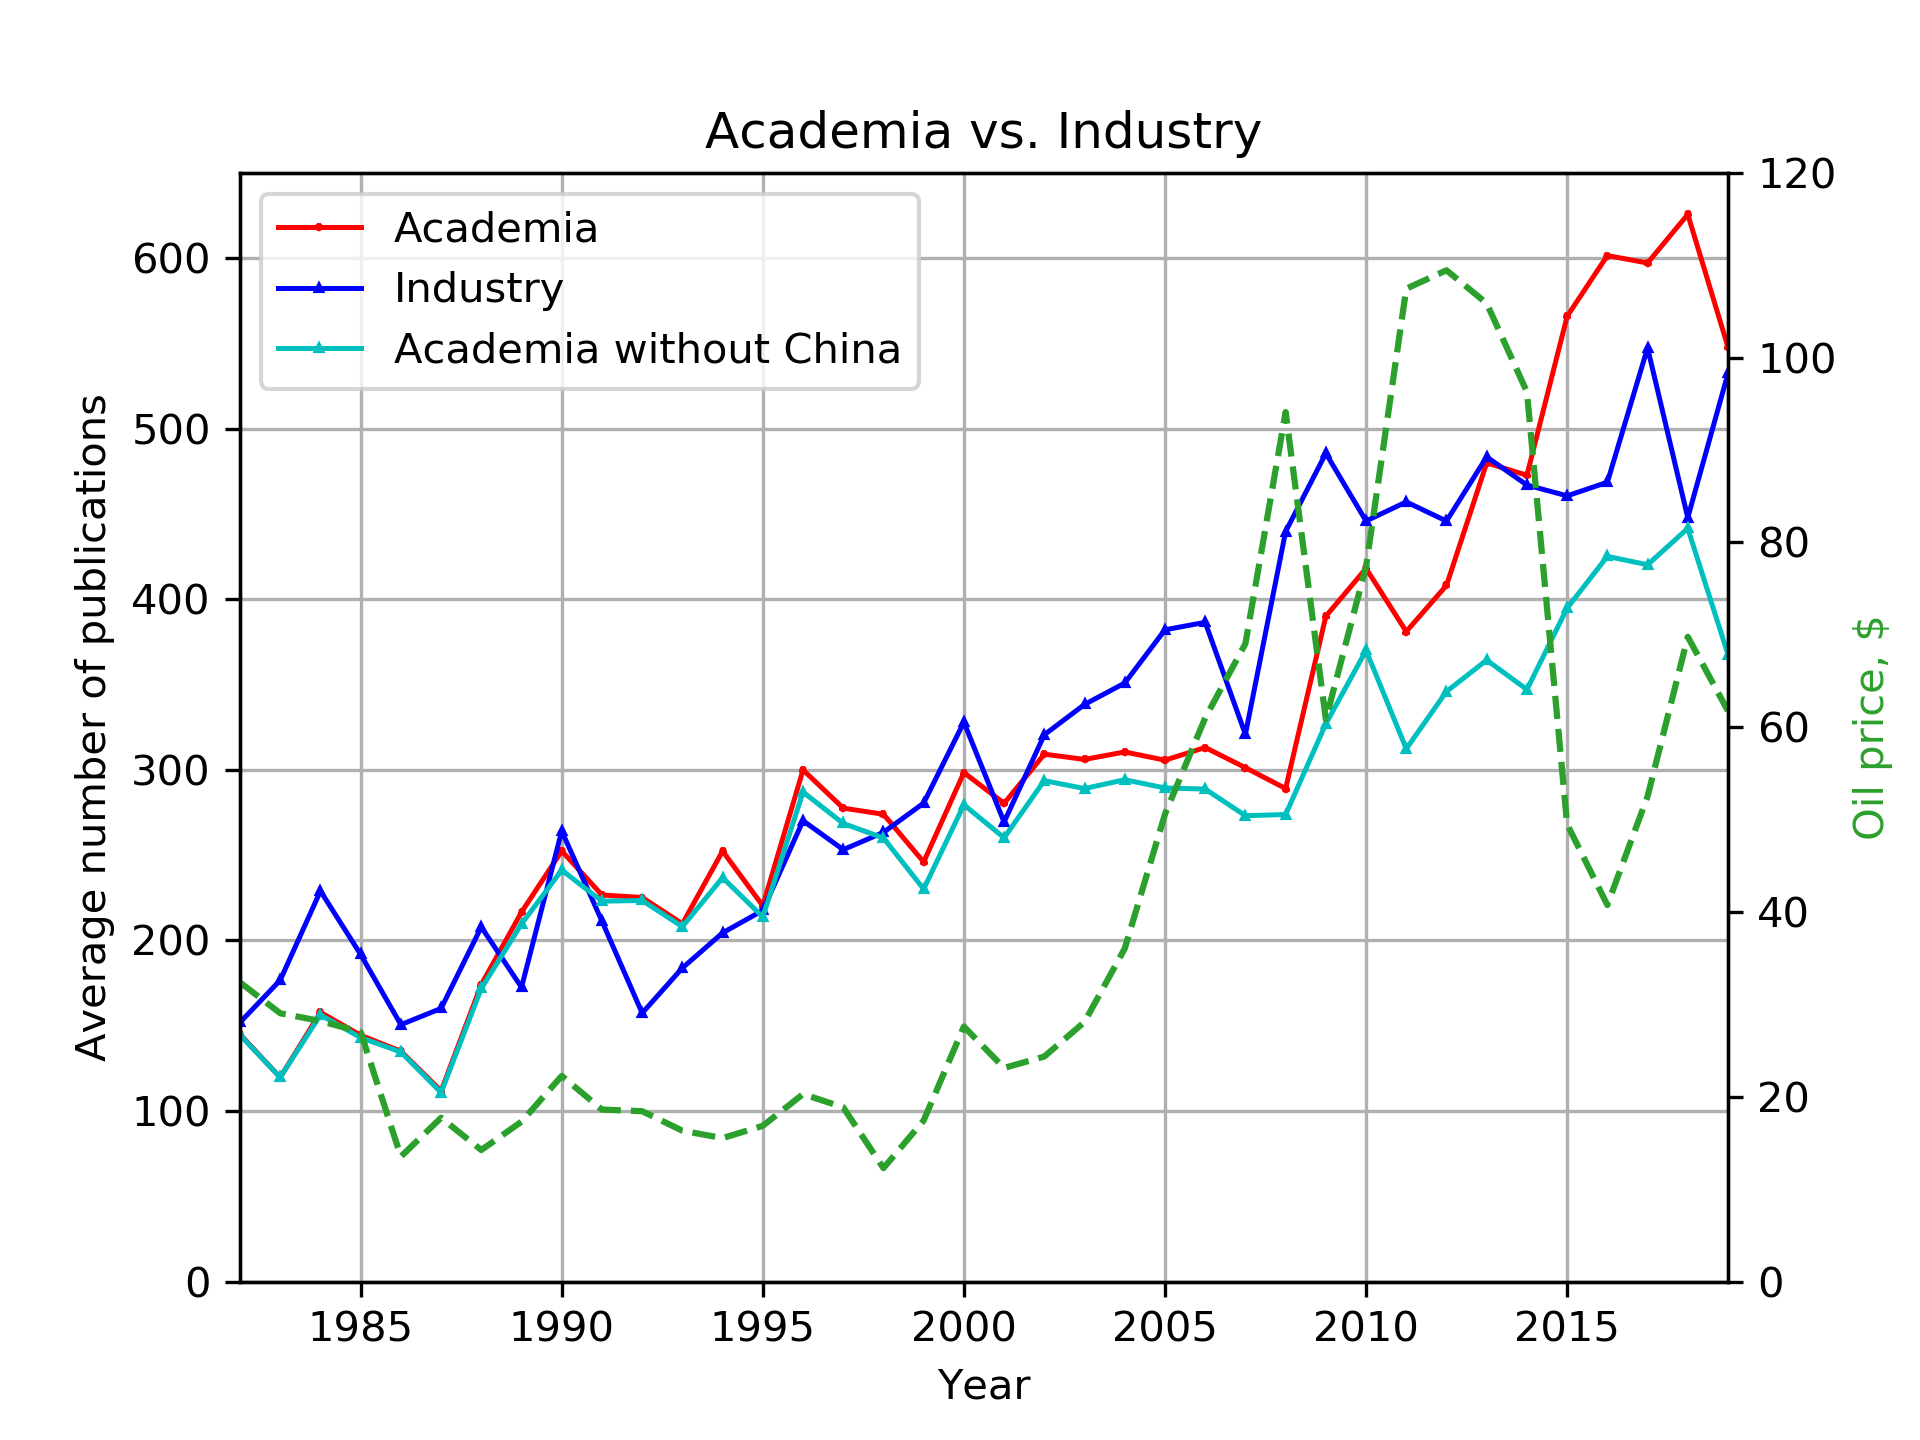
\includegraphics[scale=0.7]{acad_indus_plot.png}
\caption{Industry vs. academia average publications.}
\label{acad_vs_ind}
\end{figure}

Fig. \ref{acad_vs_ind} breakdown comparison of industry and academia impact: from 1982 to 1988, the industry was the leader in the number of publications, from 1989 to 1991 they made approximately the same contribution. From 1991 to 1994, the academia went ahead in the number of publications, for which from 1995 to 2002 there was approximately the same contribution. From 2003 to 2013, again, most of the publications are observed from the industry, this period is replaced by an increase in publications from the academia from 2014 to 2019. You can notice the correspondence of the growth trend in oil prices with the number of publications from both the academia and the industry. Local peaks in oil prices in 1990, 1996, 2000 are displayed in an increase in number of publications from industry and academia. A steady increase in oil prices from 2001 to 2008 has a general trend with an increase in the number of publications from the industry at the same period of time. While the peak in oil prices in 2008 with a subsequent drop is repeated for the industry in 2009 and in 2010 for the number of publications from the academia. An increase in oil prices from 2009 with a subsequent fall from 2012 to 2016 is reflected in an increase in the number of publications and a fall from the academia from 2014 to 2019, with a significant time lag.


It is curious that the number of publications from the academia in the last year has fallen significantly. Fig. \ref{acad_vs_ind} indicates a decrease in publications in 2019 compared to 2018 from the USA academia. Perhaps this was due to a decrease in state funding of higher educational institutions, \citep{Brownstein2018}.

After 2014, the number of academic affiliations has increased significantly and continues to grow.  While contribution from the industry has almost flattened out. The academia performance can be explained by the development of geophysics in China (see corresponding lines in Fig. \ref{acad_vs_ind}).  Industry seems to never fully recover from the 2008 crisis and then hit by the crisis of 2014.

Analysis of co-author number also provides interesting insights. Figure \ref{co_auth} shows that the number of co-authors per paper increases and we observe a correlation with the world trend in the earth and planetary sciences. This reflects the world trend in science that is now done in teams. The SEG average co-author number almost flattens out at 3.6 co-authors per paper, but in 2019 number of authors per paper increased reaching 3.9. Science is becoming more collective, and geophysics is no exception. The number of co-authors per paper increases, and we observe a correlation with the world trend in the earth and planetary sciences. With that we see an increase in amount of organizations involved in the SEG Annual Conference.


\begin{figure}[ht!]
\centering
\includegraphics[scale=0.7]{co_auth.png}
\caption{Increase in number of authors per paper for SEG Annual Conference and for earth and planetary science \citep{Mallapaty2018}.}
\label{co_auth}
\end{figure}


Fig. \ref{acad_countries} shows a breakdown by country to academia publications. For the whole time USA academia dominates in the number of papers. Some countries, like the Netherlands of Canada, have steady contribution, and their publication rate is constant over time. Other countries, like France or Germany, seem to follow oil price trend. In contrast, USA and China maintain steady growth rate. The number of publications from China exhibits the fastest growth rate; its contribution is now equal to USA.  If we count the number of affiliations for the entire observation period, this is what we get the USA: 15461, China: 5701, Canada: 2765 and Netherlands: 1584. It is necessary to note the increase in the number of publications from universities of Kingdom of Saudi Arabia over the past 10 years. in 2009 the average number of publications was about 1 and in 2019 it is more than 23, that is indeed impressive. None of the academies of other countries has shown such rapid relative growth in recent years.

\begin{figure}[ht!]
\centering
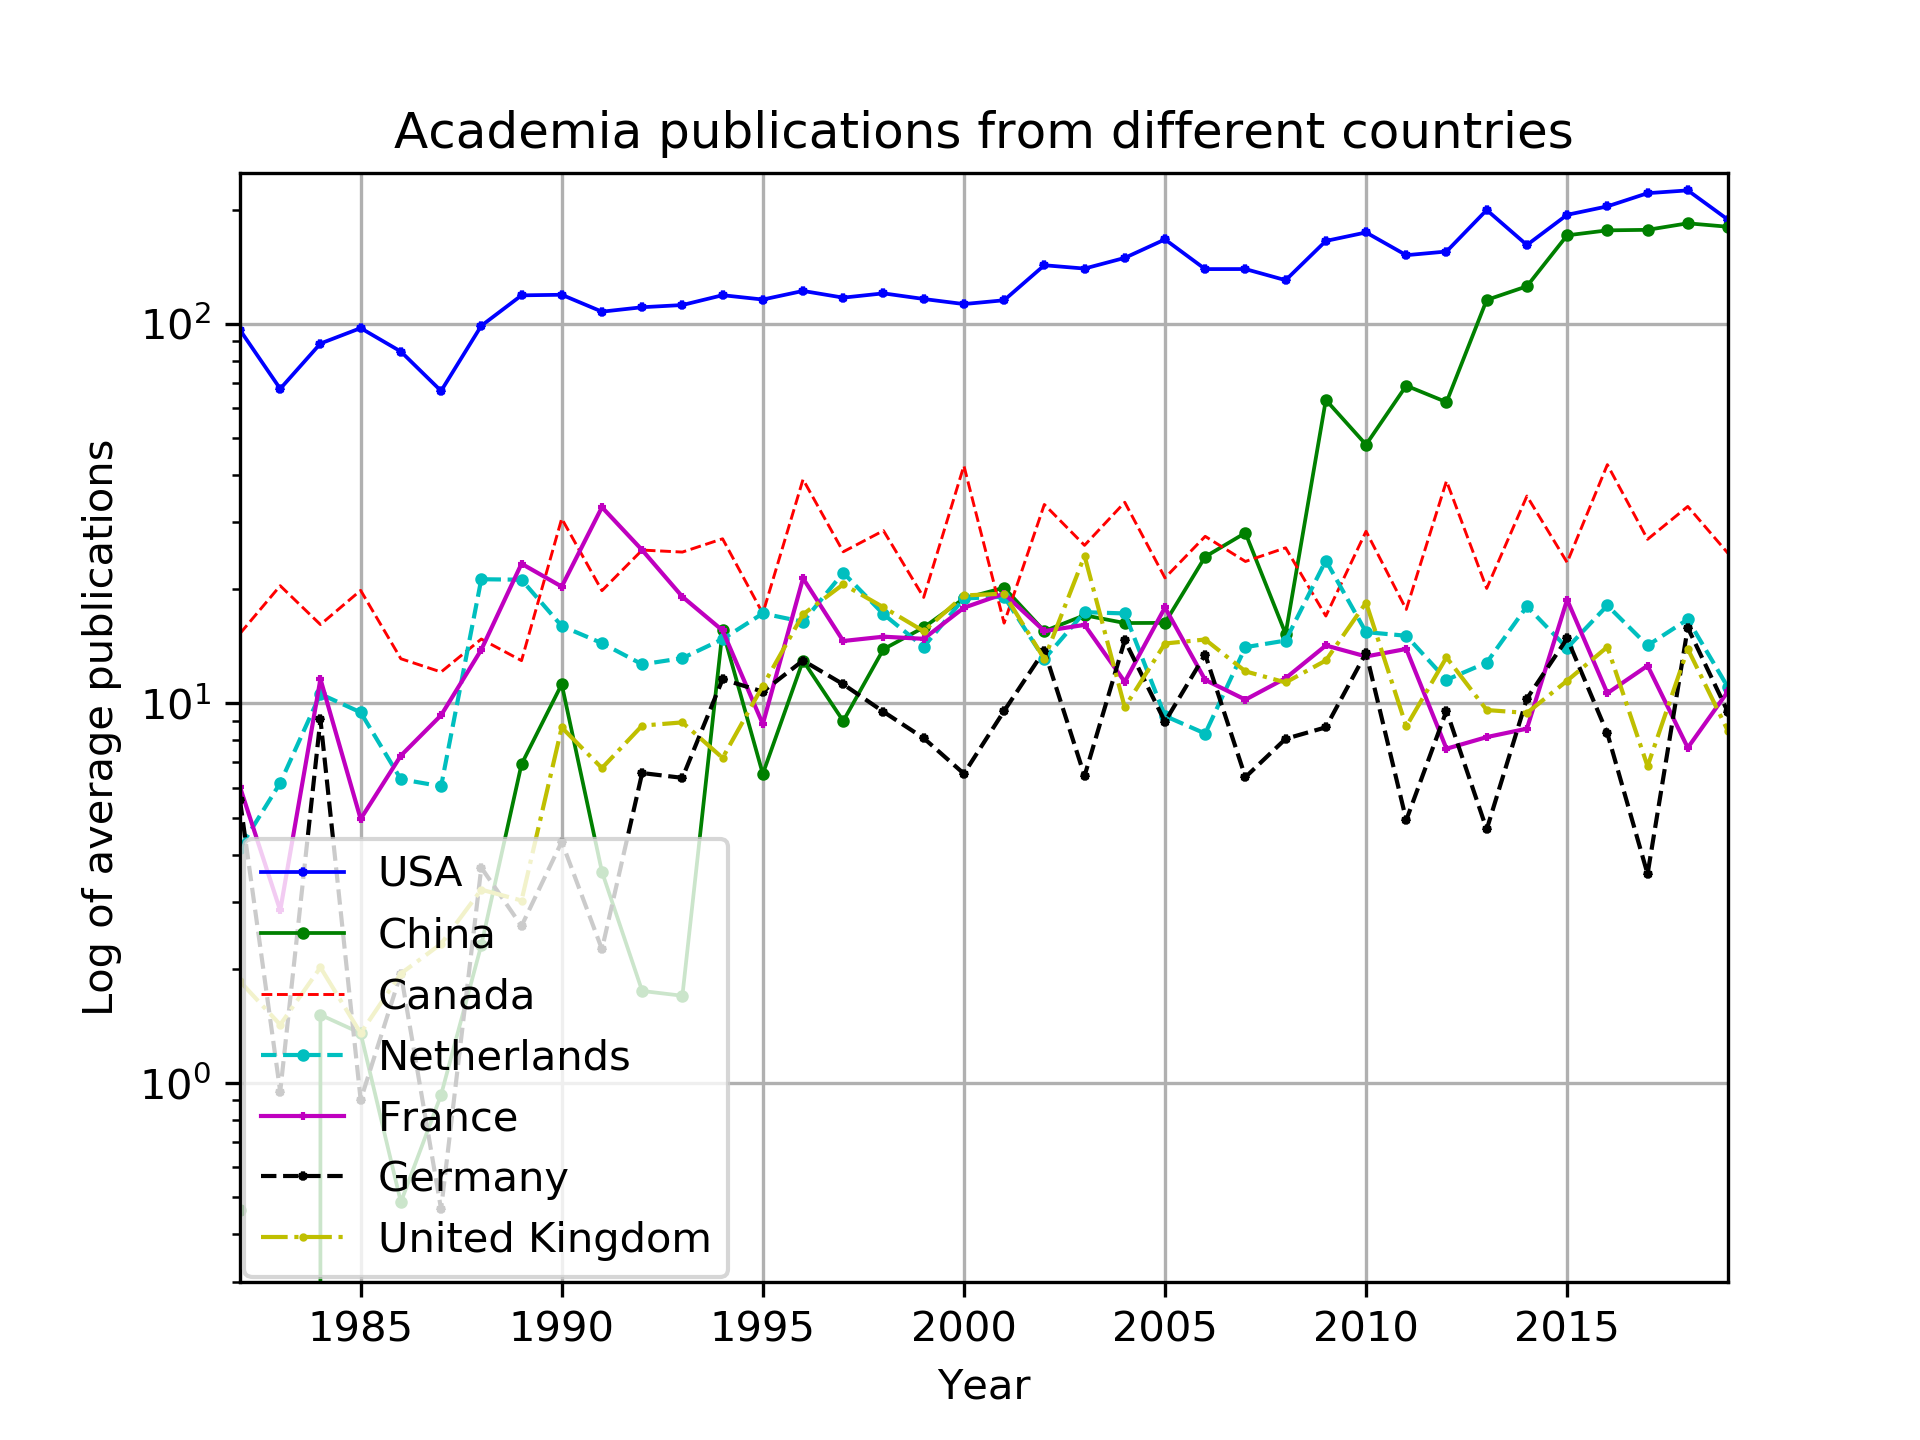
\includegraphics[scale=0.7]{acad_countries.png}
\caption{Average publications by different countries academia.}
\label{acad_countries}
\end{figure}

We next breakdown the data by industrial company contributions. Fig. \ref{oil_and_serv} shows the average number of papers by oilfield service (left) and oil company (right). The most frequent guests at the SEG Annual Conferences are Schlumberger, WesternGeco, CGG and BGP, although WesternGeco is a part of Schlumberger we are plotting them separately according to the affiliations. Basically, we see that industrial geophysics research is dominated by Schlumberger followed by CGG and BGP. In general, the number of publications by the major oilfield services contributors grows steadily. Although oilfield service companies are dependent on oil prices, we surprisingly observe that after the crisis of 2014 the number of Schlumberger publications peaked for several consecutive years, declining in 2018 and starting to grow again in 2019. The change in the number of publications from Schlumberger over the past 10 years is very similar in dynamics to the change in oil prices with a few years delay. CGG publication number follows crude oil price too but since 2014, the number of publications from CGG only declines. Number of BGP publications shows similar trend with oil prices with one or two years delay and now we see the number of publications increased last year giving BGP the leadership in 2019.

\begin{figure}[ht!]

\begin{minipage}{0.47\linewidth}
\center{\includegraphics[clip,width=1\linewidth]{Oil_service.png} }
\end{minipage}
\hfill
\begin{minipage}{0.51\linewidth}
\center{\includegraphics[clip,width=1\linewidth]{Oil_comp2.png} }
\end{minipage}

\caption{Average number of publications by oil-service and oil companies. The oil-service graph includes OPEC crude oil price.}
\label{oil_and_serv}
\end{figure}


Many oil and gas companies that no longer exist have made significant contributions to the SEG Annual Conference in the 80s and early 90s. They are Arco Oil and Gas Co., Mobil E\& P, OYO Corporation, Statoil, and others. These companies merged with others, or larger companies bought them. We are more interested in existing companies, and on the Fig. \ref{oil_and_serv} one can observe five oil companies with the biggest number of publications.  The picture is conceptually different from oilfield service companies. For example, number of publications by BP and ExxonMobil peaked in 2005 and nowadays is in decline.  For example, in 2014, we found only one paper from ExxonMobil, which has not happened over the past 15 years.  Summary Annual Report 2014 \citep{ExxonMobil2014} shows that compared to 2013 market valuation at the end of the year decreased by 12\%, and we observe the decline in the stock market price of the ExxonMobil in 2015. Hardly anyone will deny that with a decrease in profits, companies are primarily cut back on the financing of research in general and business trips to conferences in particular. This means that the absence of the company at the conference is caused by economic problems and investors can use this information to make a profit. Saudi Aramco demonstrates a steady growth, it had the biggest number of publications of all production companies in 2017 and 2018. Interestingly enough, the leadership was taken by Petrochina in 2019 followed by Shell and Saudi Aramco is on the third place.


\subsection{Technical term analysis}
In this section we present our analysis of the manuscript texts from SEG Annual Conference. However, instead of focusing on average text length or sentence complexity, we look into technical side. For example, we analyze and compare frequency of occurrence of technical terms, such like data, velocity, etc. Such an analysis sheds some light on technology development and trends in the field.

Fig. \ref{grams} shows that the most commonly used words, two- and three-words phrases that appeared in conference materials over during 38 years. The most common words are “data,” “model,” “velocity,” “seismic.” The word “data” was mentioned more than 377700 times, “seismic” – 252400, “model” more than 251500 times and “velocity” more than 223300 times in thirty-eight years. For comparison the mention of word “that” was 324250 times.  Most of three- and two-words phrases are devoted to seismic exploration and seismic data processing. 

\begin{figure}[ht!]

\begin{minipage}{0.24\linewidth}
\center{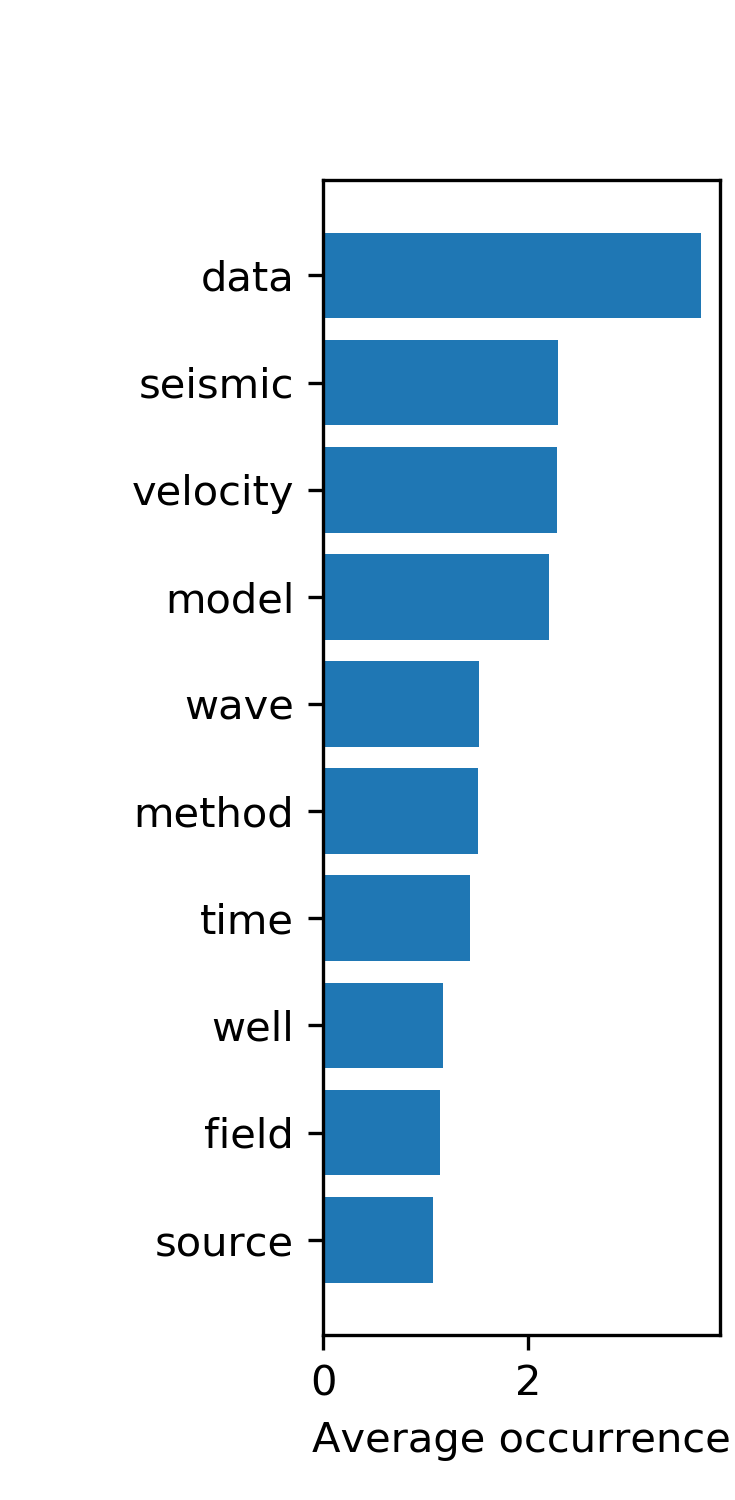
\includegraphics[clip,width=1\linewidth]{sigrams.png} }
\end{minipage}
\hfill
\begin{minipage}{0.329\linewidth}
\center{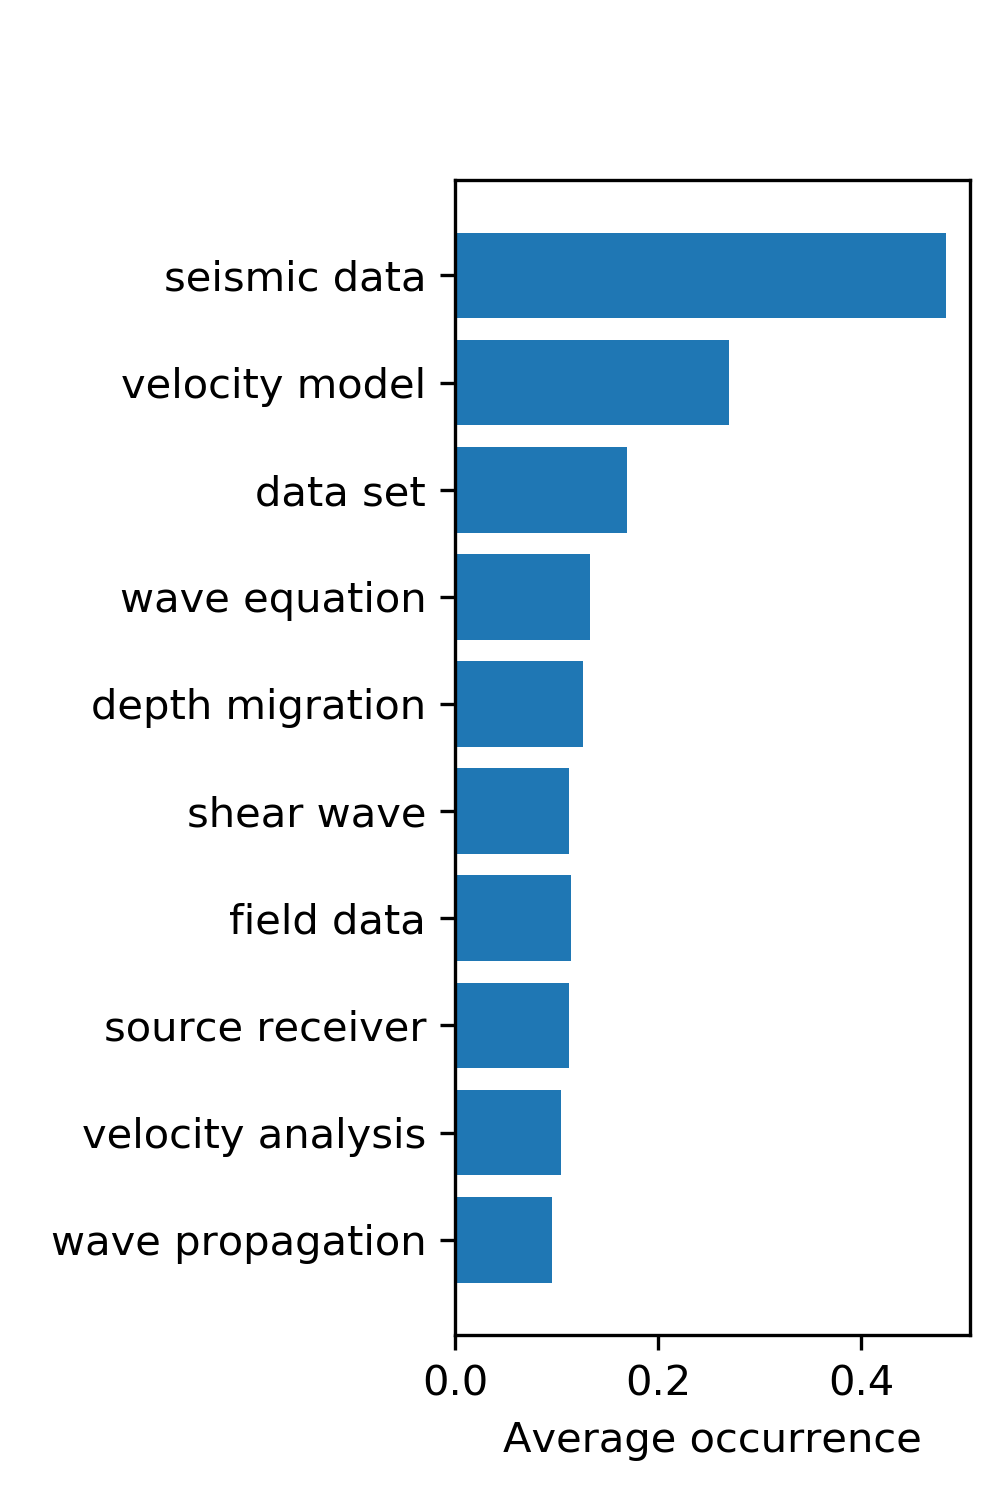
\includegraphics[clip,width=1\linewidth]{bigrams.png} }
\end{minipage}
\hfill
\begin{minipage}{0.4\linewidth}
\center{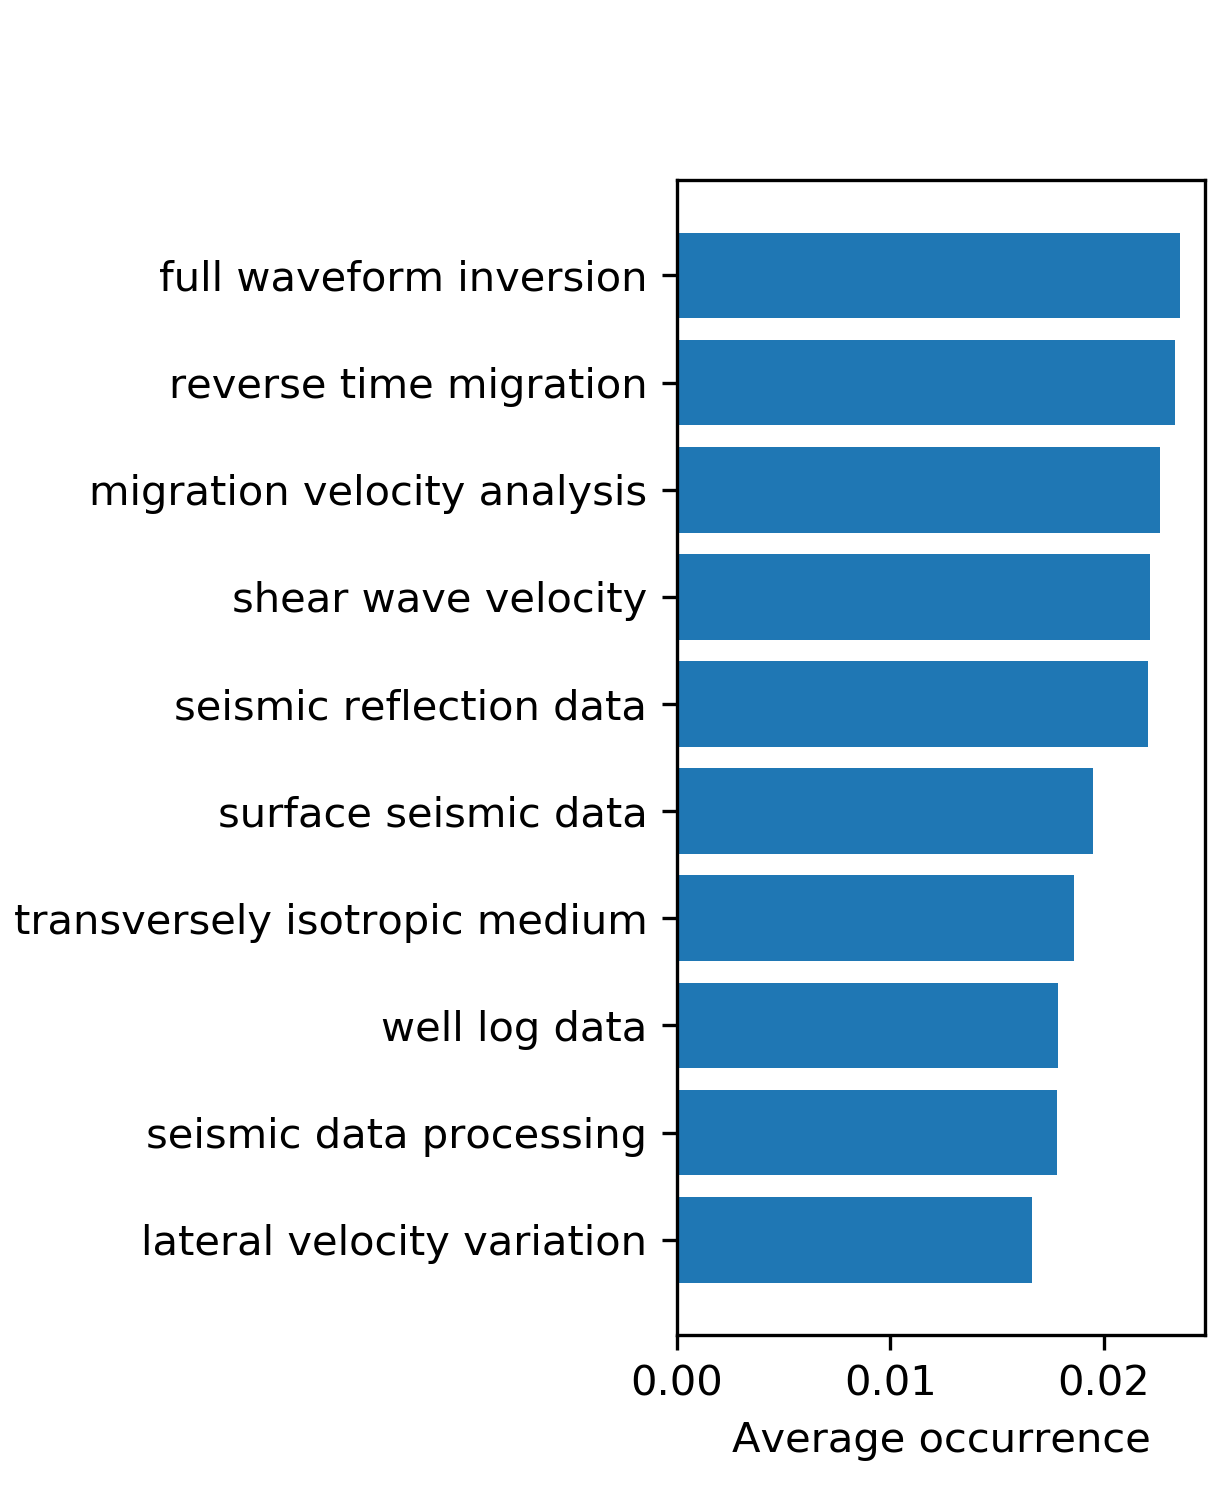
\includegraphics[clip,width=1\linewidth]{trigrams.png} }
\end{minipage}

\caption{The most common words and phrases of two and three word.}
\label{grams}
\end{figure}


Frequent use of these words tells us that most of the articles are about seismic exploration and seismic data processing. Such words as “wellbore” and “logging” were more popular during the 1980s and now their relative occurrence is declining. We normalize the data to the number of pages of all articles; one should consider it as the number of words used per page of text per year.  Such a normalization will be the most correct: if we check the usage of most frequent English words (the, of, and, to, etc.), the average number of their uses per page remains unchanged over the last decades, and it can be a reliable reference. There was no significant change in the number of words per page during the study period. 

\begin{figure}[ht!]
\centering
\includegraphics[scale=0.7]{rocks.png}
\caption{Most occurred names of rocks}
\label{rocks}
\end{figure}
 
Fig. \ref{rocks} shows the distribution of the names of rocks used in time. Fig. \ref{rocks} reflects the “shale” revolution and the decline of more traditional sandstone reservoirs. In turn, “volcanic” rocks throughout history were about the same used except for the early 1980s, and they start to occur more in the past few years. It is worth noting that the frequency use of words "sandstone" and "carbonate" is really close as for "limestone" and "volcanic". The interest in shale is understandable, the amount of hydrocarbon reserves is huge %add link
, while they are difficult to extract, which forces research. Fig. \ref{shales_frac} shows most often used names of shale reserves on the left and on the right we see usage of "fracking", it includes "hydraulic fracturing", "frac", and "fracking" and "shale gas" + "gas shale". We definitely observe peaking of shale related terms from 2010 to 2015, which was followed by a decline in recent few years. The use of the words "fracturing" and "shale gas" is unlikely to decrease in the near future. Fig. \ref{shales_frac} shows peaking of shale related words between 2010 and 2016. In the past 20 years "Barnett" shale mentioned more frequent than other shale. In 2019 "Marcellus", "Eagle" (Ford), and "Barnett" show the same occurrence, about 1 time per 100 pages. 
On the right one can see that after the increase in 2010, "fracking" and "shale gas" are still used frequent. The oil and gas reserves in the shale are huge,% add a link
 but they are difficult to extract. It can be assumed that the tendency will remain similar. It is clear that shale gas will not solve all the energy problems of mankind, but we will need this resource.   

“Inversion” is increasing in frequency of occurrence and now it is ~2 times per page, while in mid-1990 it was about one time per page.  It seems logical as seismic inversion takes a lot of computational power and gives a better image of the underground structure; the use of inversion increased with the appearance of technical means. 

\begin{figure}[ht!]

\begin{minipage}{0.49\linewidth}
\center{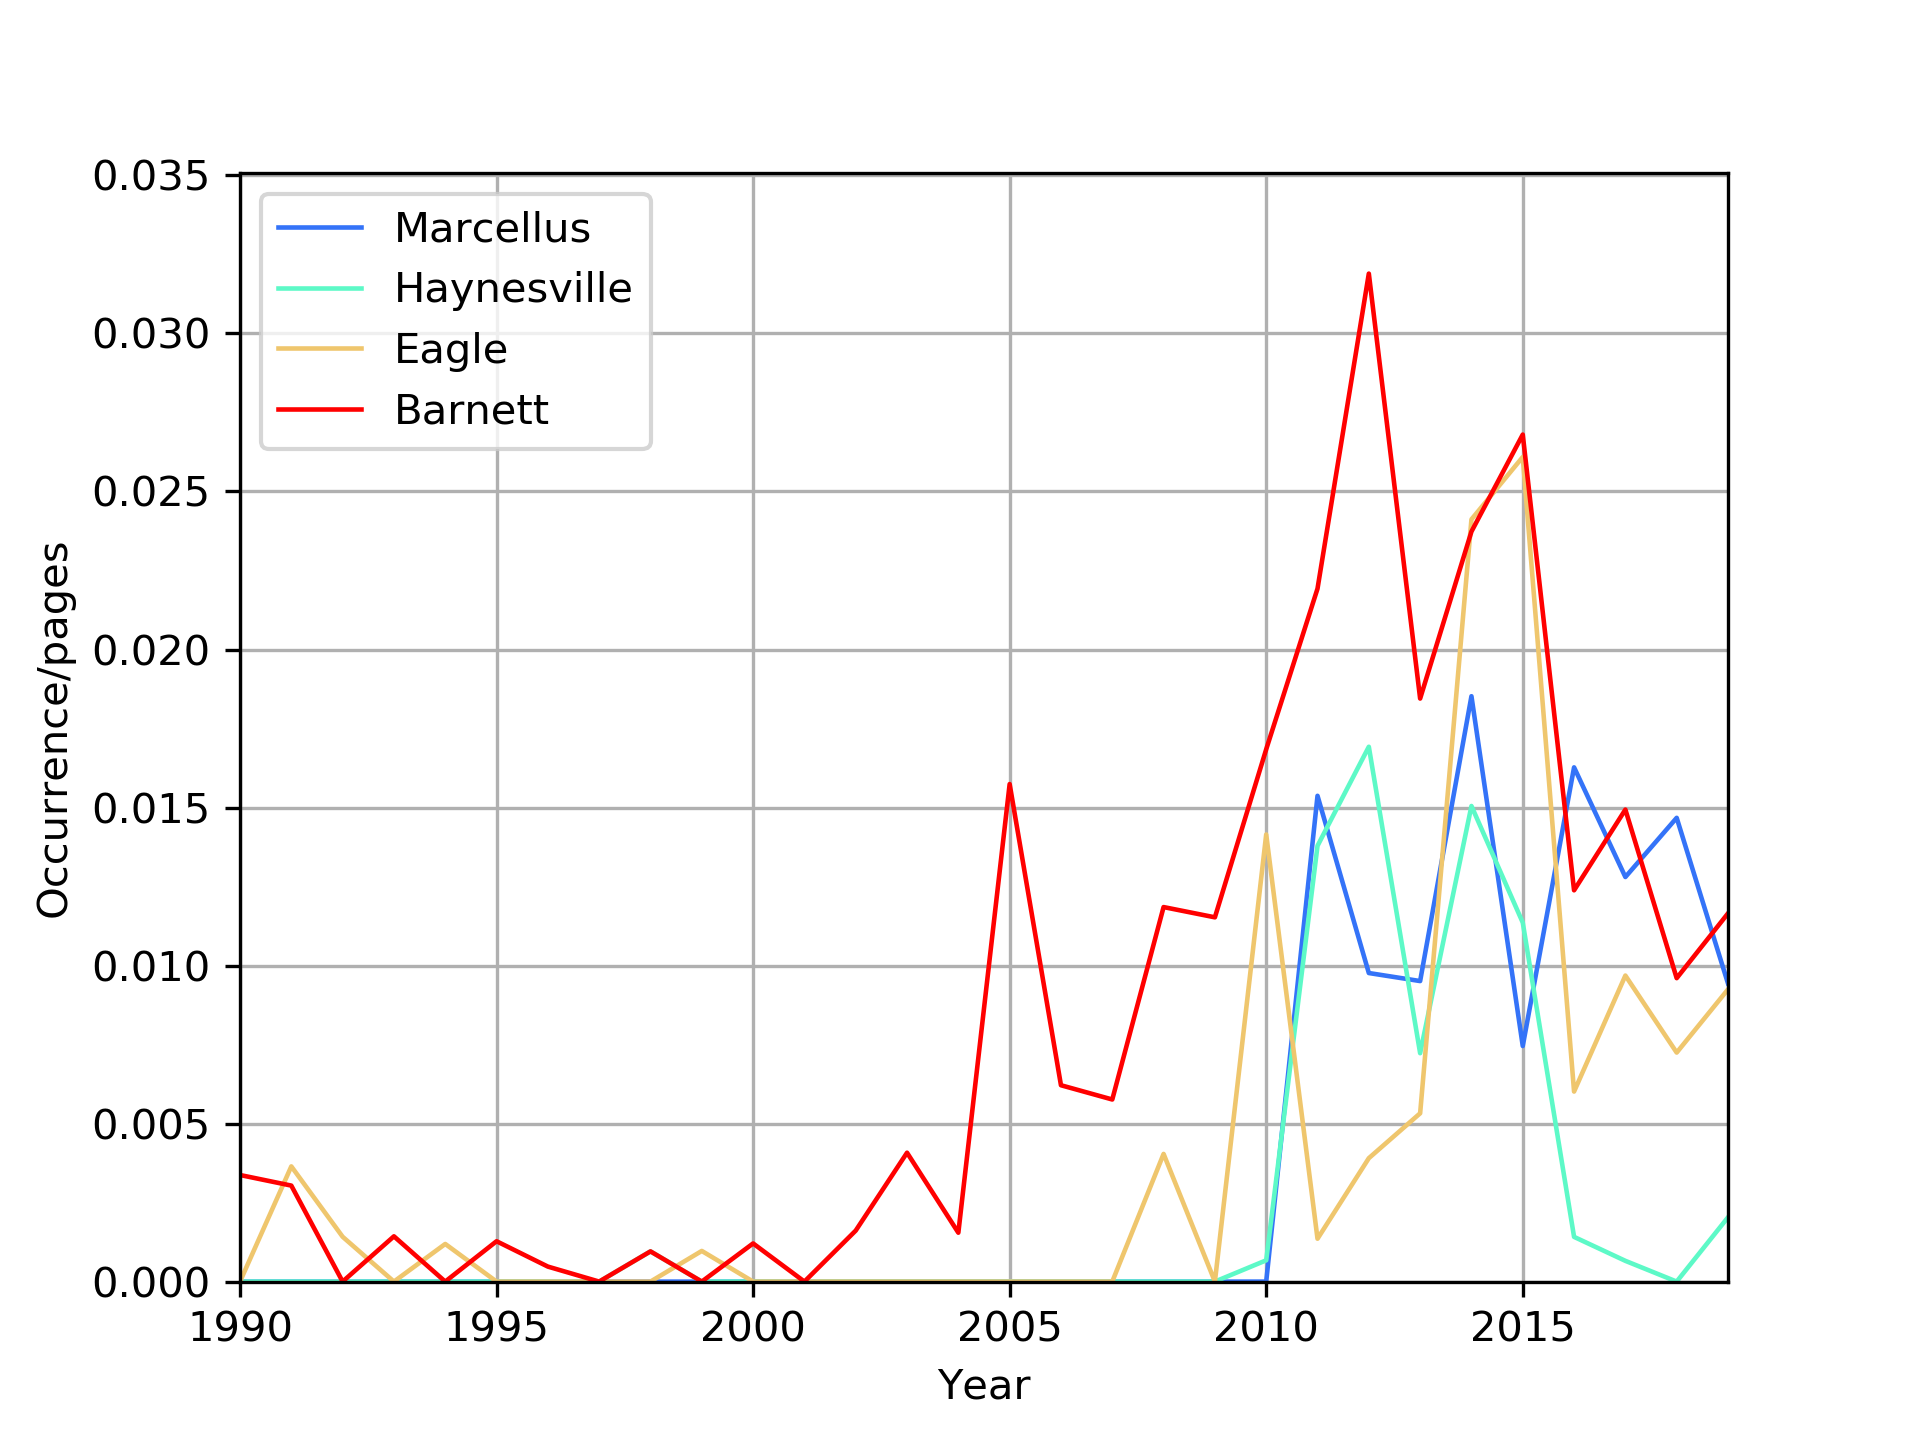
\includegraphics[clip,width=1\linewidth]{shales.png} }
\end{minipage}
\hfill
\begin{minipage}{0.49\linewidth}
\center{\includegraphics[clip,width=1\linewidth]{shale_frac.png} }
\end{minipage}

\caption{Left - most occured shale reserves; right -  frequency of hydraulic fracturing and shale gas.}
\label{shales_frac}
\end{figure}


For the past 14 years we see a trend of decreasing in frequency of occurrence of word “survey”, it is worth noting that in the past two years there has been a local increase in the use of this term, perhaps this is due to the shale deposits and now it is about 0.53 times per page which is still a lot. We see an increase in the use of word “monitoring” during almost all the 38 years, and now it reaches 0.17 times per page. We assume that the trend will continue because the number of mineral depositions is limited, and it is impossible to do an infinite survey. Probably we will observe more articles related to “monitoring” of explored fields.


\begin{figure}[ht!]

\begin{minipage}{0.49\linewidth}
\center{\includegraphics[clip,width=1\linewidth]{neurald_fieldd.png} }
\end{minipage}
\hfill
\begin{minipage}{0.49\linewidth}
\center{\includegraphics[clip,width=1\linewidth]{nn.png} }
\end{minipage}

\caption{Neural network related two-word phrases, "field data" phrase was taken as a reference.}
\label{neur_netw}
\end{figure}

More interesting to know what terms are gaining popularity now and what are the current trends in geophysics. Let's consider words increased in occurrence over the past two-three years. Here are the three-words phrases that gain a high rate of occurrence in 2016-2019: “deep neural network,”  processing system,” “convolutional neural network.” Fig. \ref{neur_netw} shows the appearance of “neural network,” “deep learning,” “artificial intelligence” and “field data,”  we use the last one for the reference as it is always often used. In 2019, “neural network,” occurred more often than “field data.” It has already happened during the history, in 1993 and from 1999 to 2001, after that, it declined for a while but now “neural network,” “deep learning” and “artificial intelligence” started to grow again (“artificial intelligence” appeared during 1980-s). A question is if the growth will continue or will decline again like in 1993 -1995. The decline in interest in neural networks in early 2000 can be explained by an insufficient amount of computing power to realize the capabilities of the method. Now, technological progress allows much more, neural networks are successfully used mainly for face recognition, but we see attempts to introduce them into other areas of life. It is not necessary to be a rocket scientist to understand the reasons for the increasing interest in neural networks in geophysics. Experts want to automate the geophysical data processing as much as possible. It remains only to understand whether we need to deeply automate the seismic data processing because with time we have fewer oilfields to be explored, providing space for monitoring and increasing production efficiency.
 
Fig. \ref{sigrams} shows words with the highest growth of occurrence on the left and highest rate of decline on the right. As one can observe, majority of growing in occurrence words are related to neural network method. Is it possible to assume that these words will continue to gain popularity in the upcoming years, and the topic will remain relevant? For example the phrases “streamer em” and “receiver deghosting” grown in occurrence very fast during 2011 – 2015 but since 2015 they decline as quickly as they were growing before. The word “fiber” and “fibre” is increasing in use almost as rapidly; this refers to fiber optics because seismic sensors based on fiber optics are now growing in use, showing their effectiveness in detecting faults filled with geothermal fluids \citep{Trainor-Guitton2018}, microseismic monitoring during hydraulic fracturing \citep{Binder2019} and other applications. Term  distributed acoustic sensing (DAS) shows good correspondence with the word fiber as DAS system is based on fiber-optics and these terms are used together. Here the use of the term is directly related to the production of the corresponding equipment. Unlike the subject of “neural network,” where you can use the existing computing power for development and solve the problem by writing new algorithms, the development of optical fiber requires the creation of the production. However in 2019 we observe a decline in usage of word fiber. "Marchenko" are a set of data driven methods that help us to project surface seismic data to points in the subsurface, \citep{Lomas2019}. Wasserstein metrics and data augmentation are also growing in the occurrence in past three years but not that fast as Marchenko. It can be concluded that the lack of research objects forces professionals to develop processing methods and, for example, reprocess legacy data. Right picture on Fig. \ref{sigrams} shows terms that decreased in occurrence in the past four years.Interestingly, researchers have reduced interest in the use of graphics processors, as seven to eight years ago this was a trend. "Barnett" shale is one of the most well studied and the authors believe that the fading of interest in it is a natural phenomenon. It is curious that there was increased interest in basalt at the turn of the century and we observe increased interest in the early 2010s.


Besides "neural network" related terms (Fig. \ref{bigrams}) on the left side we observe increase in usage of "tight sandstone" and "igneous rock". It is interesting that for 38 years "igneous rocks" were rarely discussed, excepting 2009. In 2018 and 2019 there were several papers studying igneous rocks as they were found on Chinese and Brazilian oil fields and their acoustic and elastic properties must be considered in the reservoir characterization \citep{Penna2019}. On the right of Fig. \ref{bigrams} one can see two words phrases that show decrease in frequency of occurrence in past 4 years. Obviously, when new research topics appear, old ones will inevitably be partially or completely replaced by new ones, since the number of articles is limited every year. Gaussian beam migration was first described by Hill in 1990, it is seismic method that can image steeply dipping reflectors (more than 90 degrees) and will not produce unwanted reflections from structure in the velocity model, \citep{Hill1990}. In 1993 at SEG Annual Conference we observe several papers reporting usage of beam migration in seismic data processing. In 2001 we see and increase in number of occurrence of "beam migration", with the increase in computing capabilities, it became possible to use this method for 3D AVO analysis of small and medium-size 3D seismic surveys, \citep{Huang2001}. Interest in this method rises two more times, in 2008 and 2015. Frequency peaks appear with enviable regularity every seven or eight years. Moreover, each subsequent peak is higher than the previous one. In 1990, a new method appeared, in 1993 we observe testing on synthetic data, in 2001 the results of processing small and medium volumes of data were reported, in 2007 and 2008 the results of use at large objects in the Gulf of Mexico \citep{Ting2008}, CGGVeritas. For 25 years, we have seen the emergence of new technologies, testing and application in field exploration. This is reflected in the frequency of use of terms in a professional language. However, since 2015, we see a decrease in the frequency of use of this term. Fig. \ref{bigrams}, we also see a decrease in the use of other seismic terms and Barnett shale.


\begin{figure}[ht!]

\begin{minipage}{0.49\linewidth}
\center{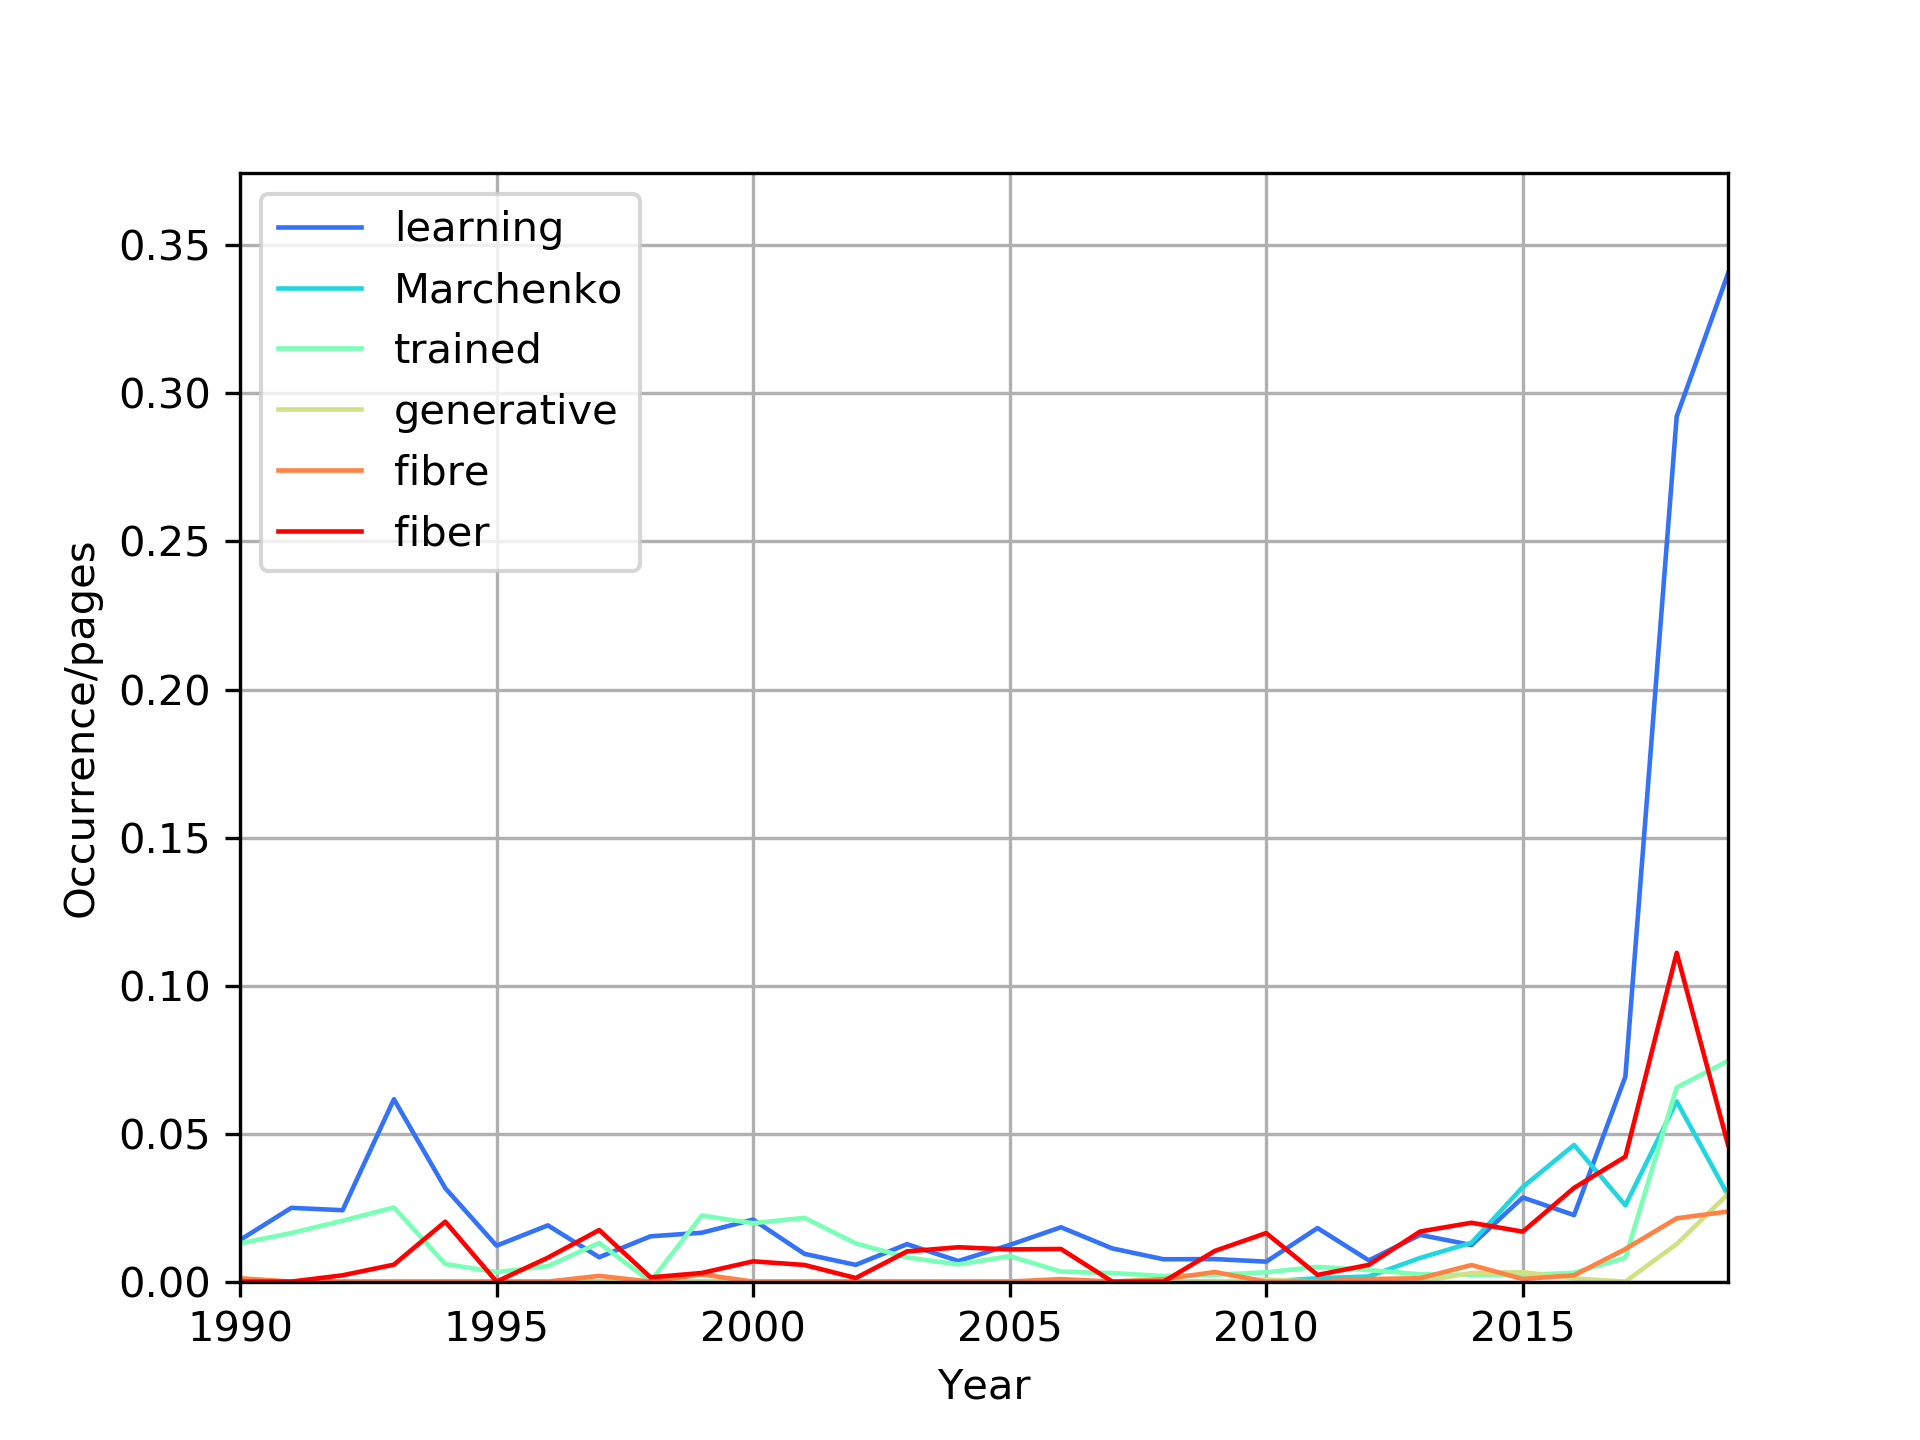
\includegraphics[clip,width=1\linewidth]{most_grow_si.png} }
\end{minipage}
\hfill
\begin{minipage}{0.49\linewidth}
\center{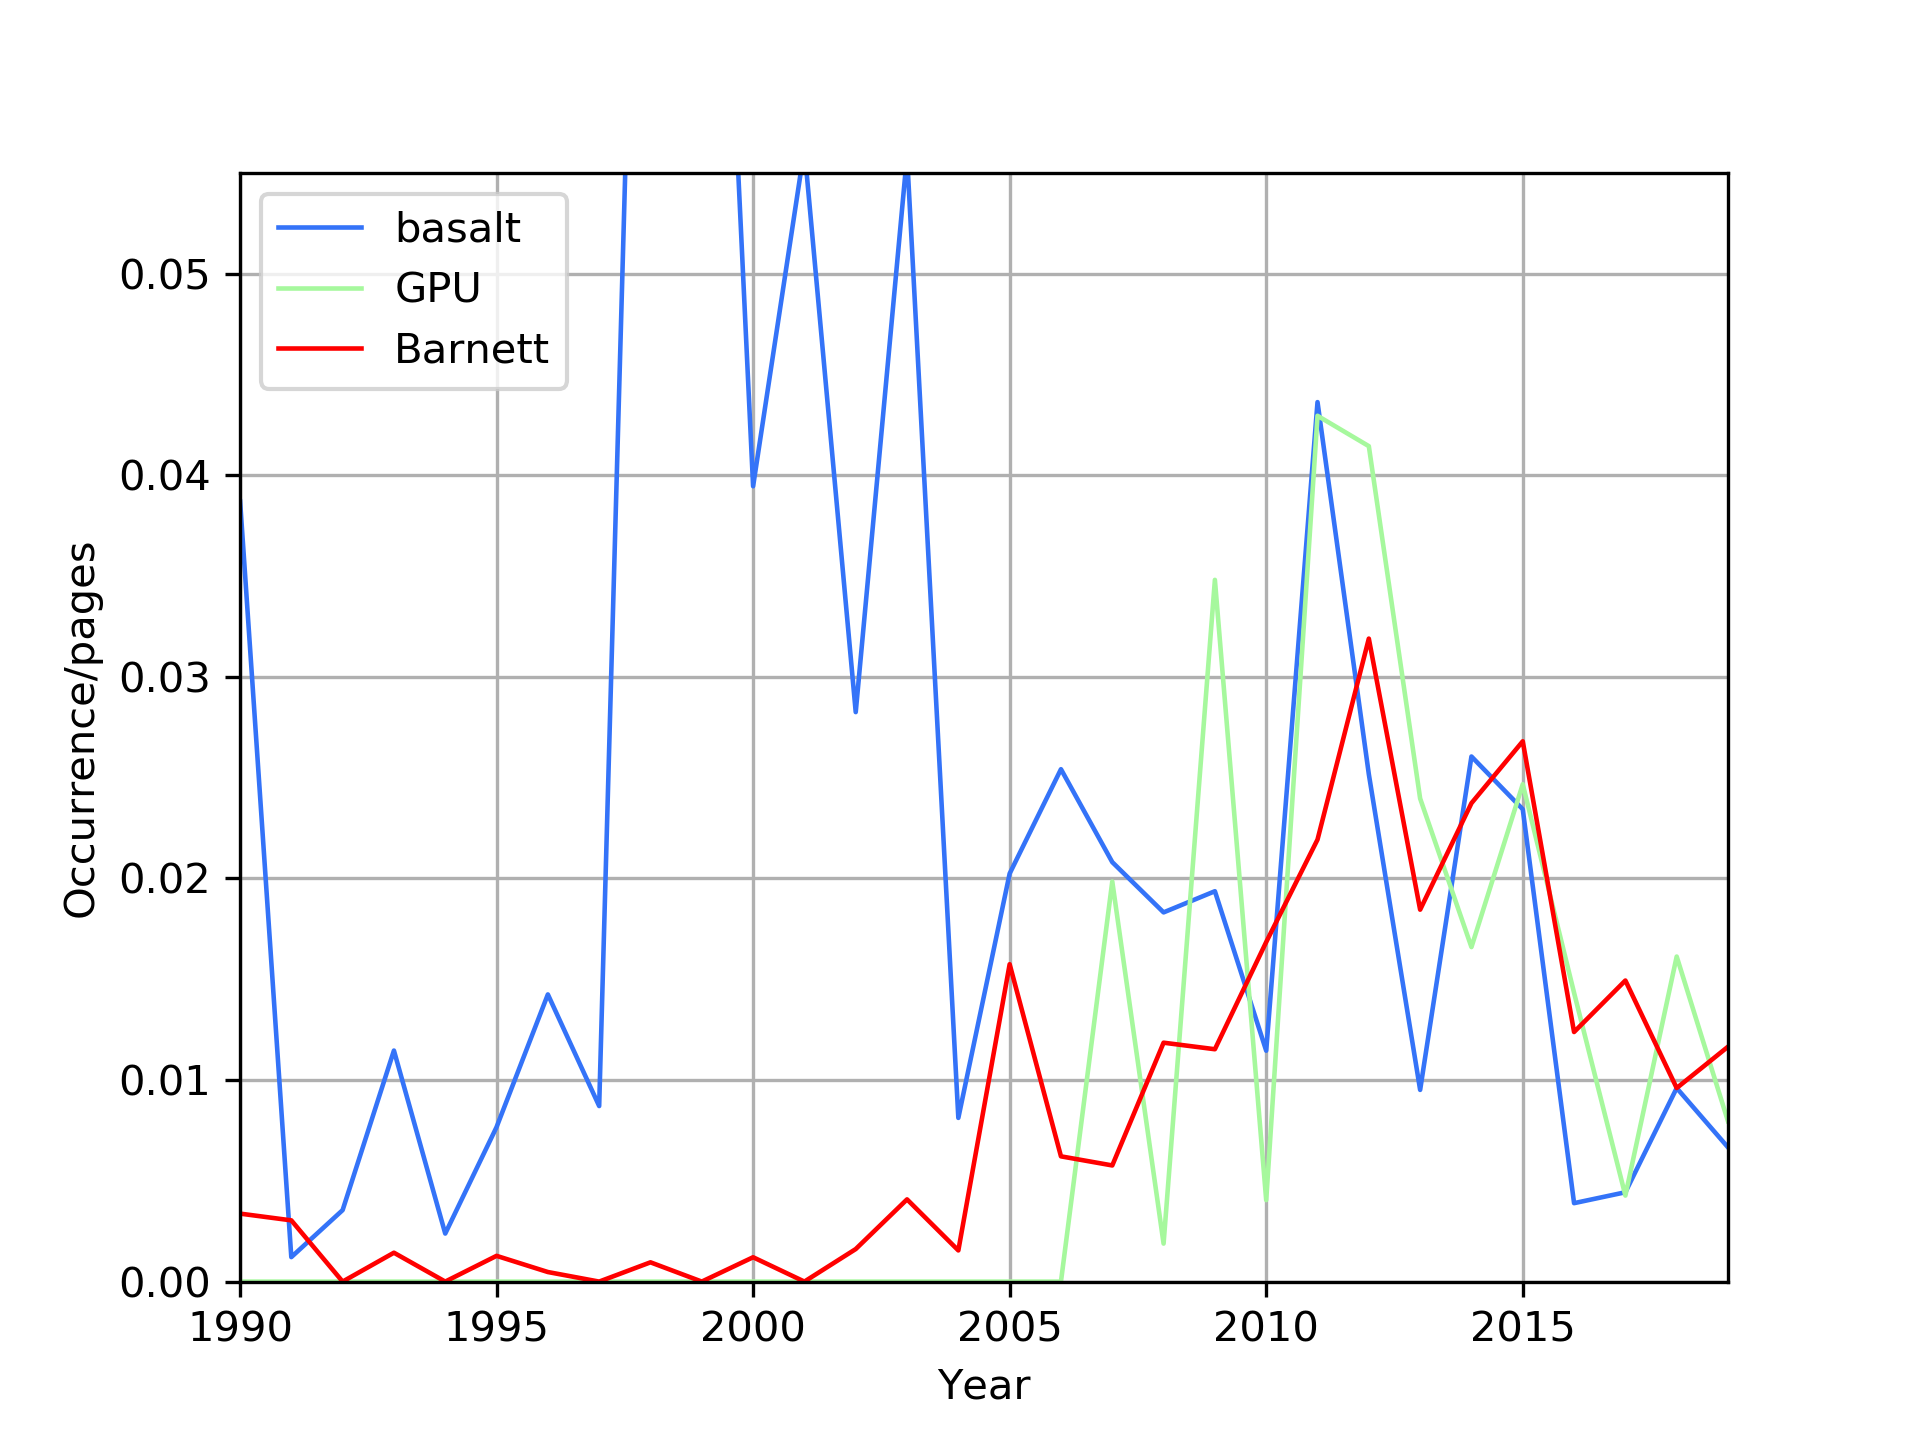
\includegraphics[clip,width=1\linewidth]{most_decl_si.png} }
\end{minipage}

\caption{Words that shows the highest rate of occurrence growth (left)  and decline (right) in the past four years.}
\label{sigrams}
\end{figure}

\begin{figure}[ht!]

\begin{minipage}{0.49\linewidth}
\center{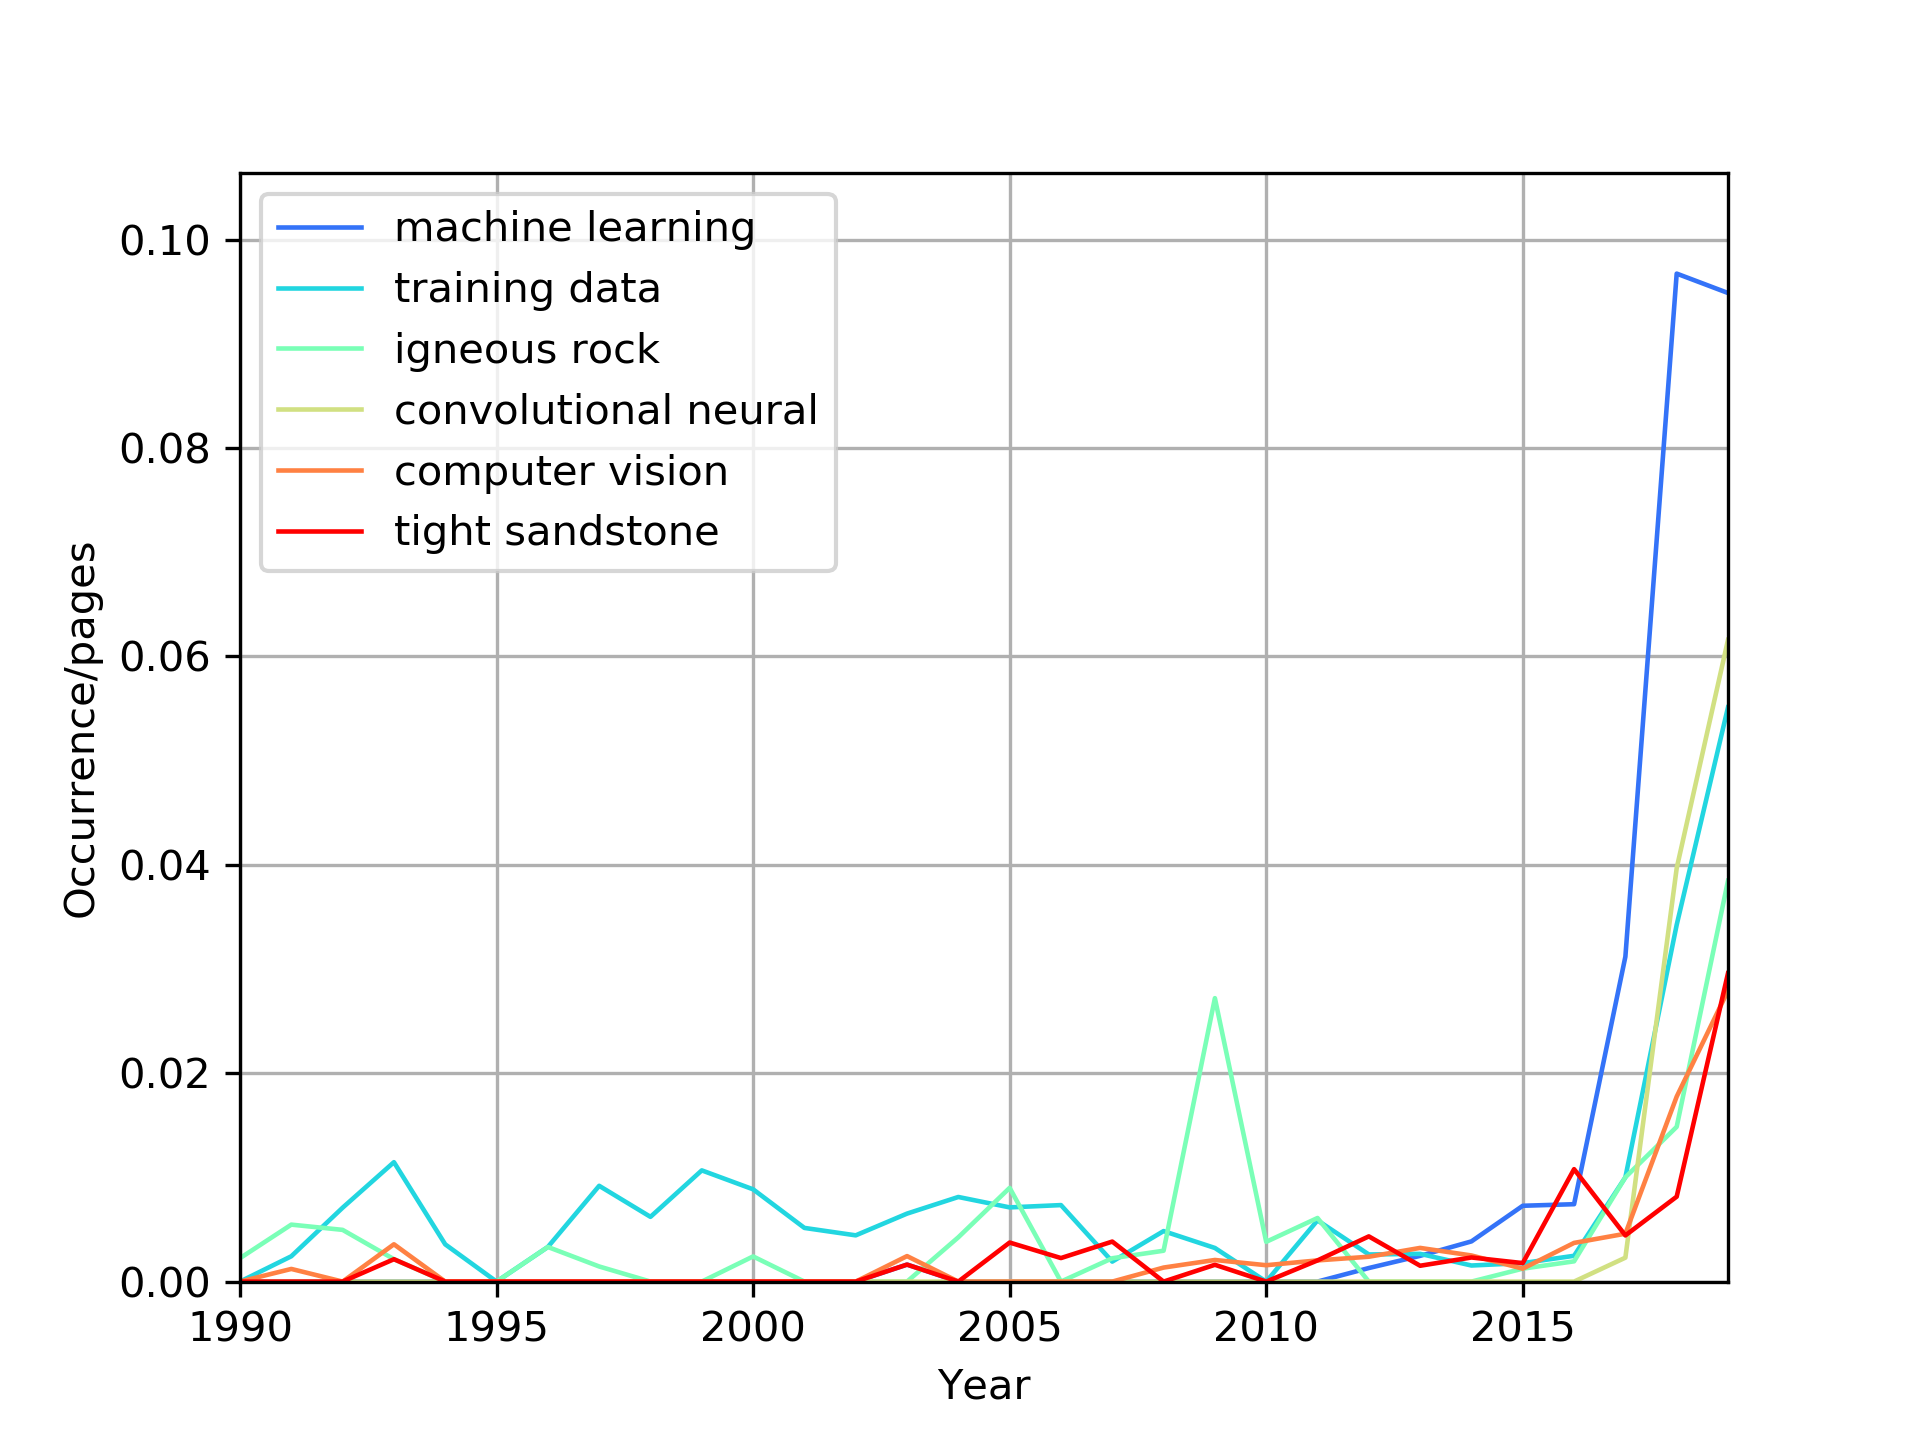
\includegraphics[clip,width=1\linewidth]{most_grow_bi.png} }
\end{minipage}
\hfill
\begin{minipage}{0.49\linewidth}
\center{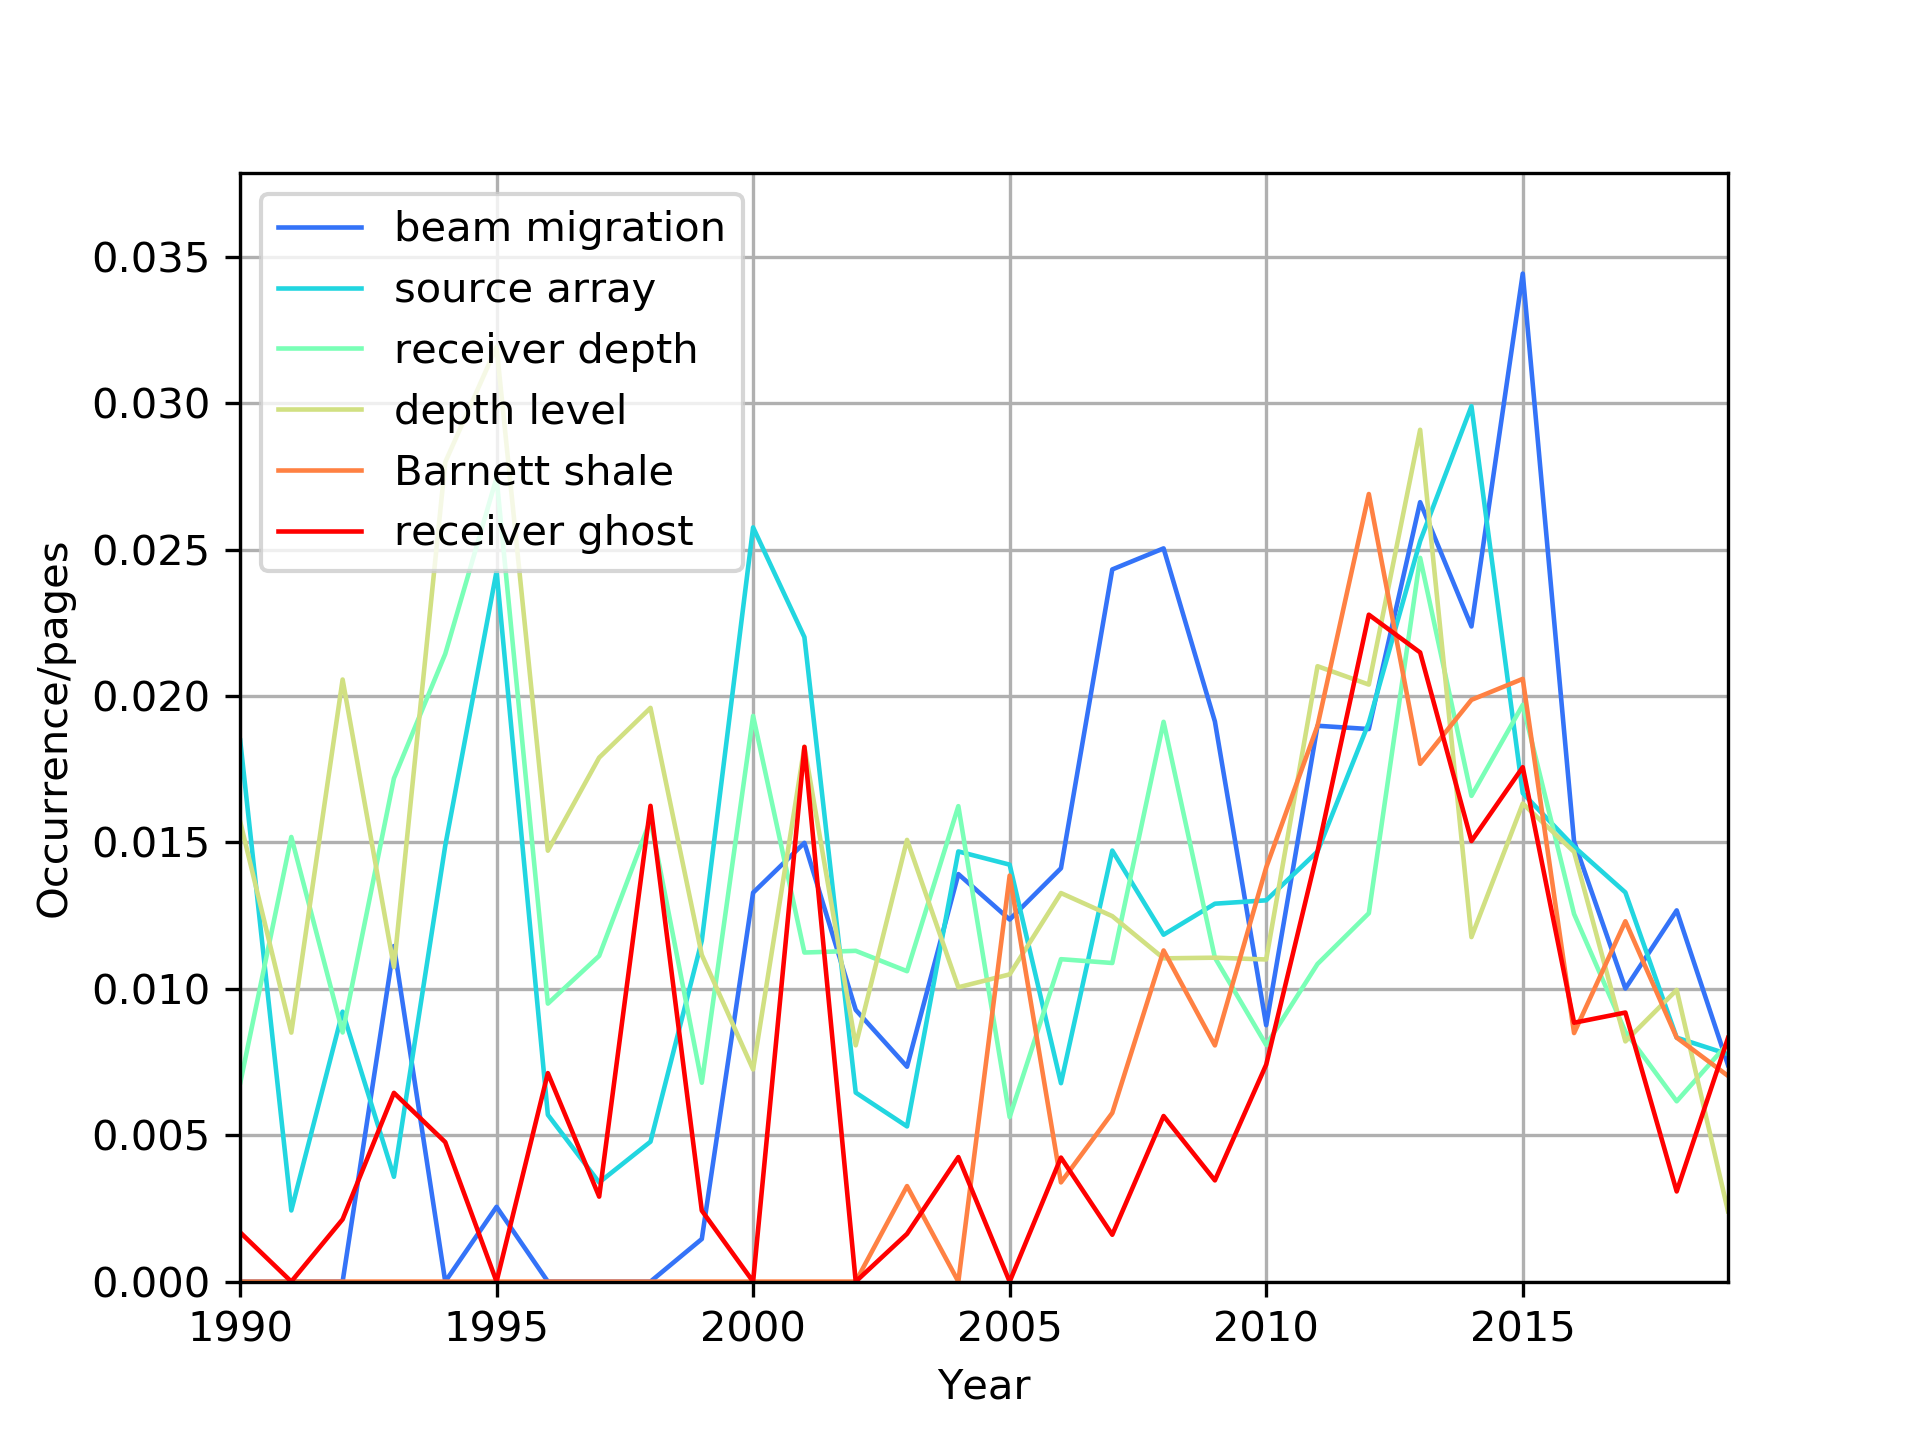
\includegraphics[clip,width=1\linewidth]{most_decl_bi.png} }
\end{minipage}

\caption{Two-words phrases that shows the highest rate of occurrence growth (left)  and decline (right) in the past four years.}
\label{bigrams}
\end{figure}


\begin{figure}[ht!]

\begin{minipage}{0.49\linewidth}
\center{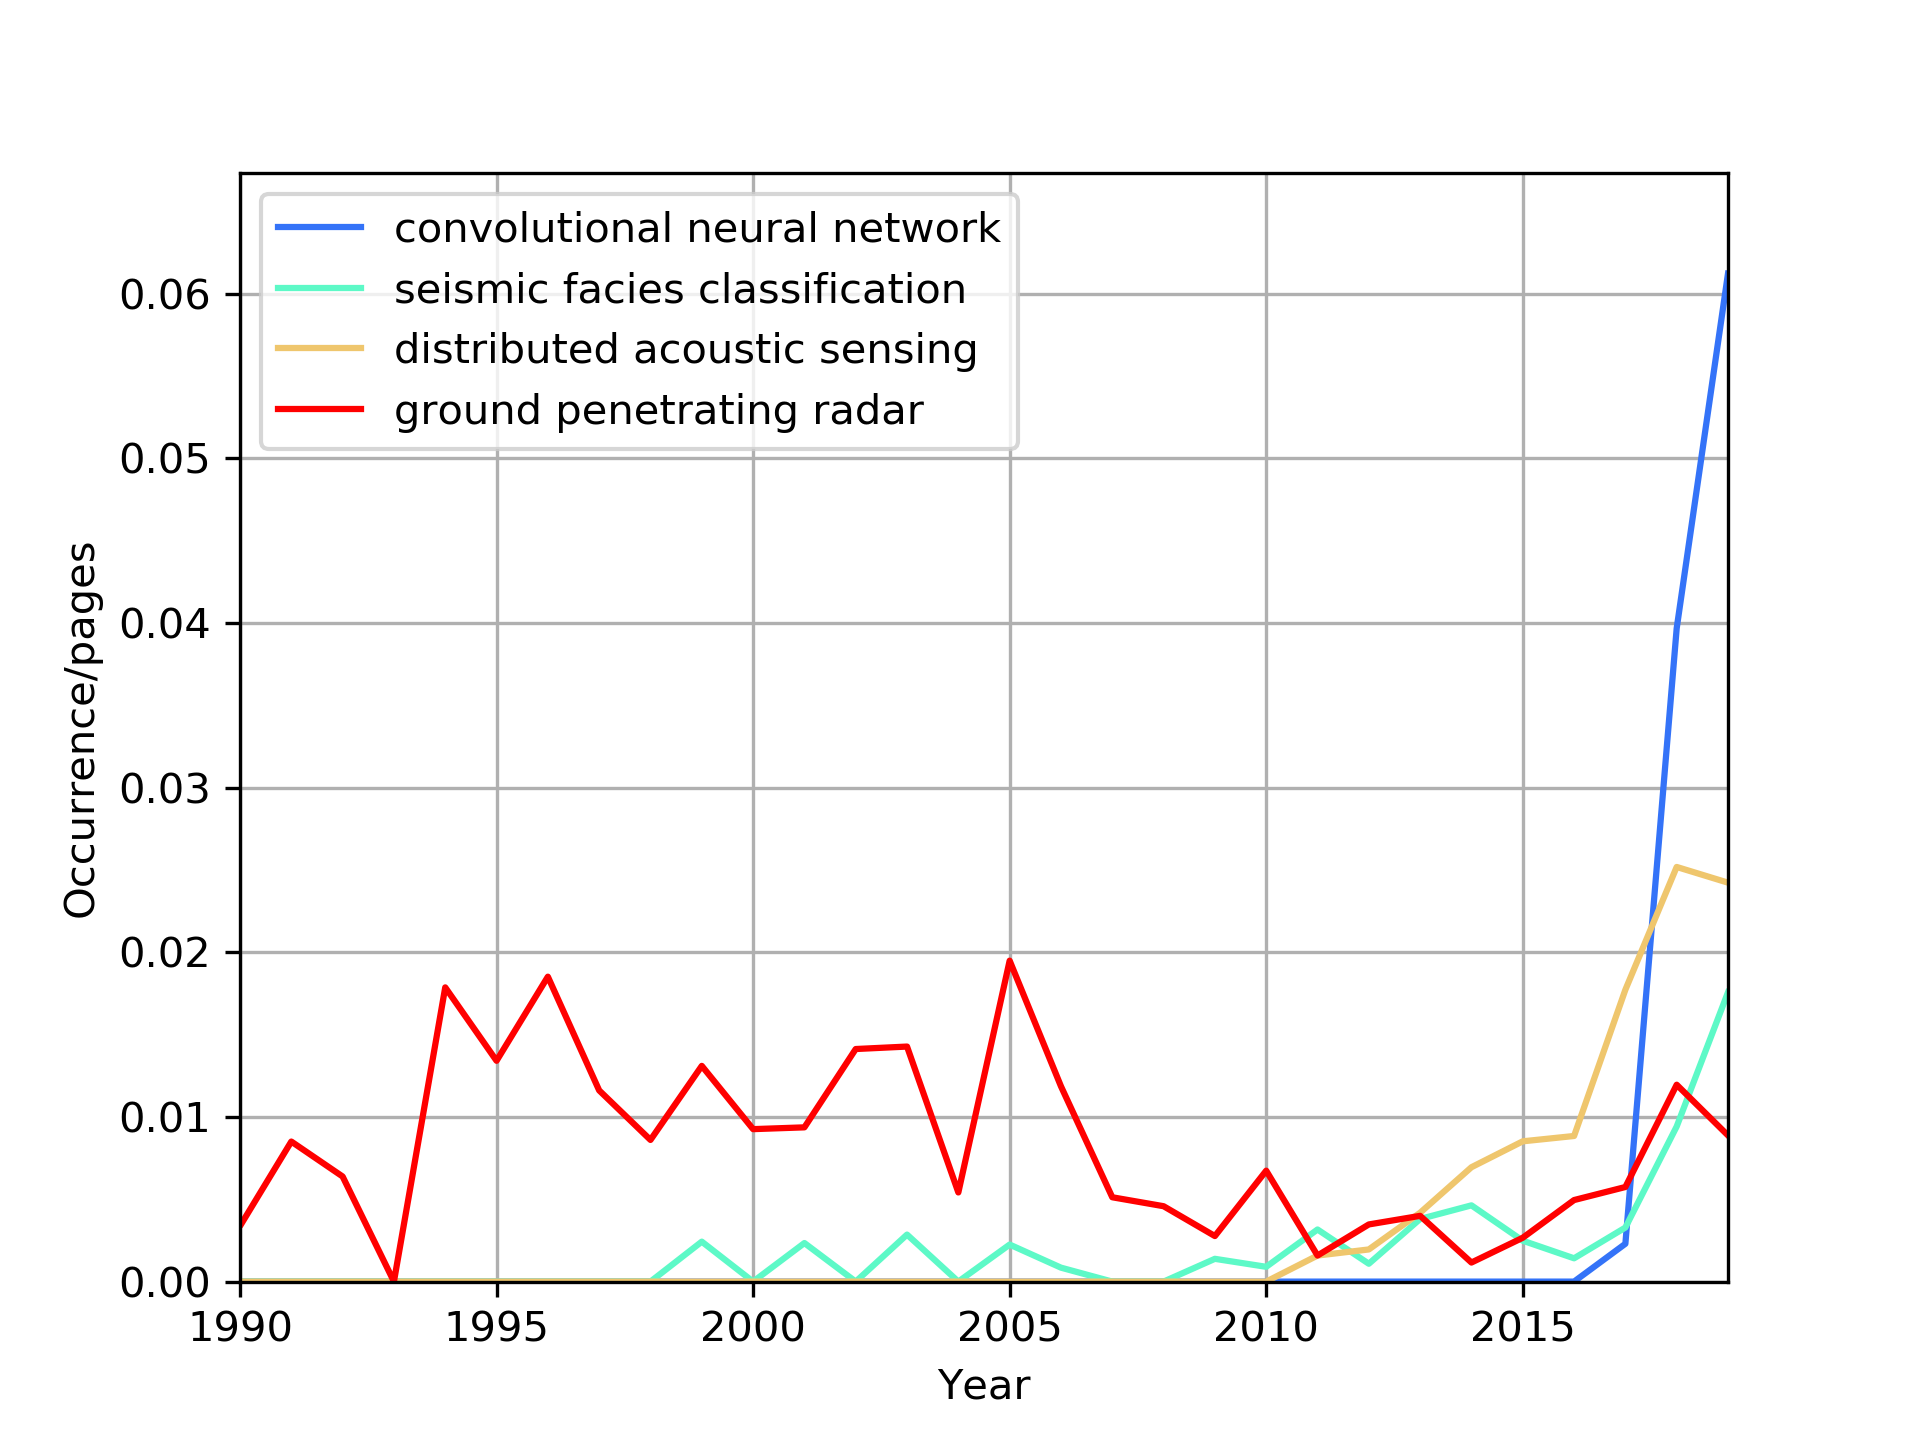
\includegraphics[clip,width=1\linewidth]{most_grow_tri.png} }
\end{minipage}
\hfill
\begin{minipage}{0.49\linewidth}
\center{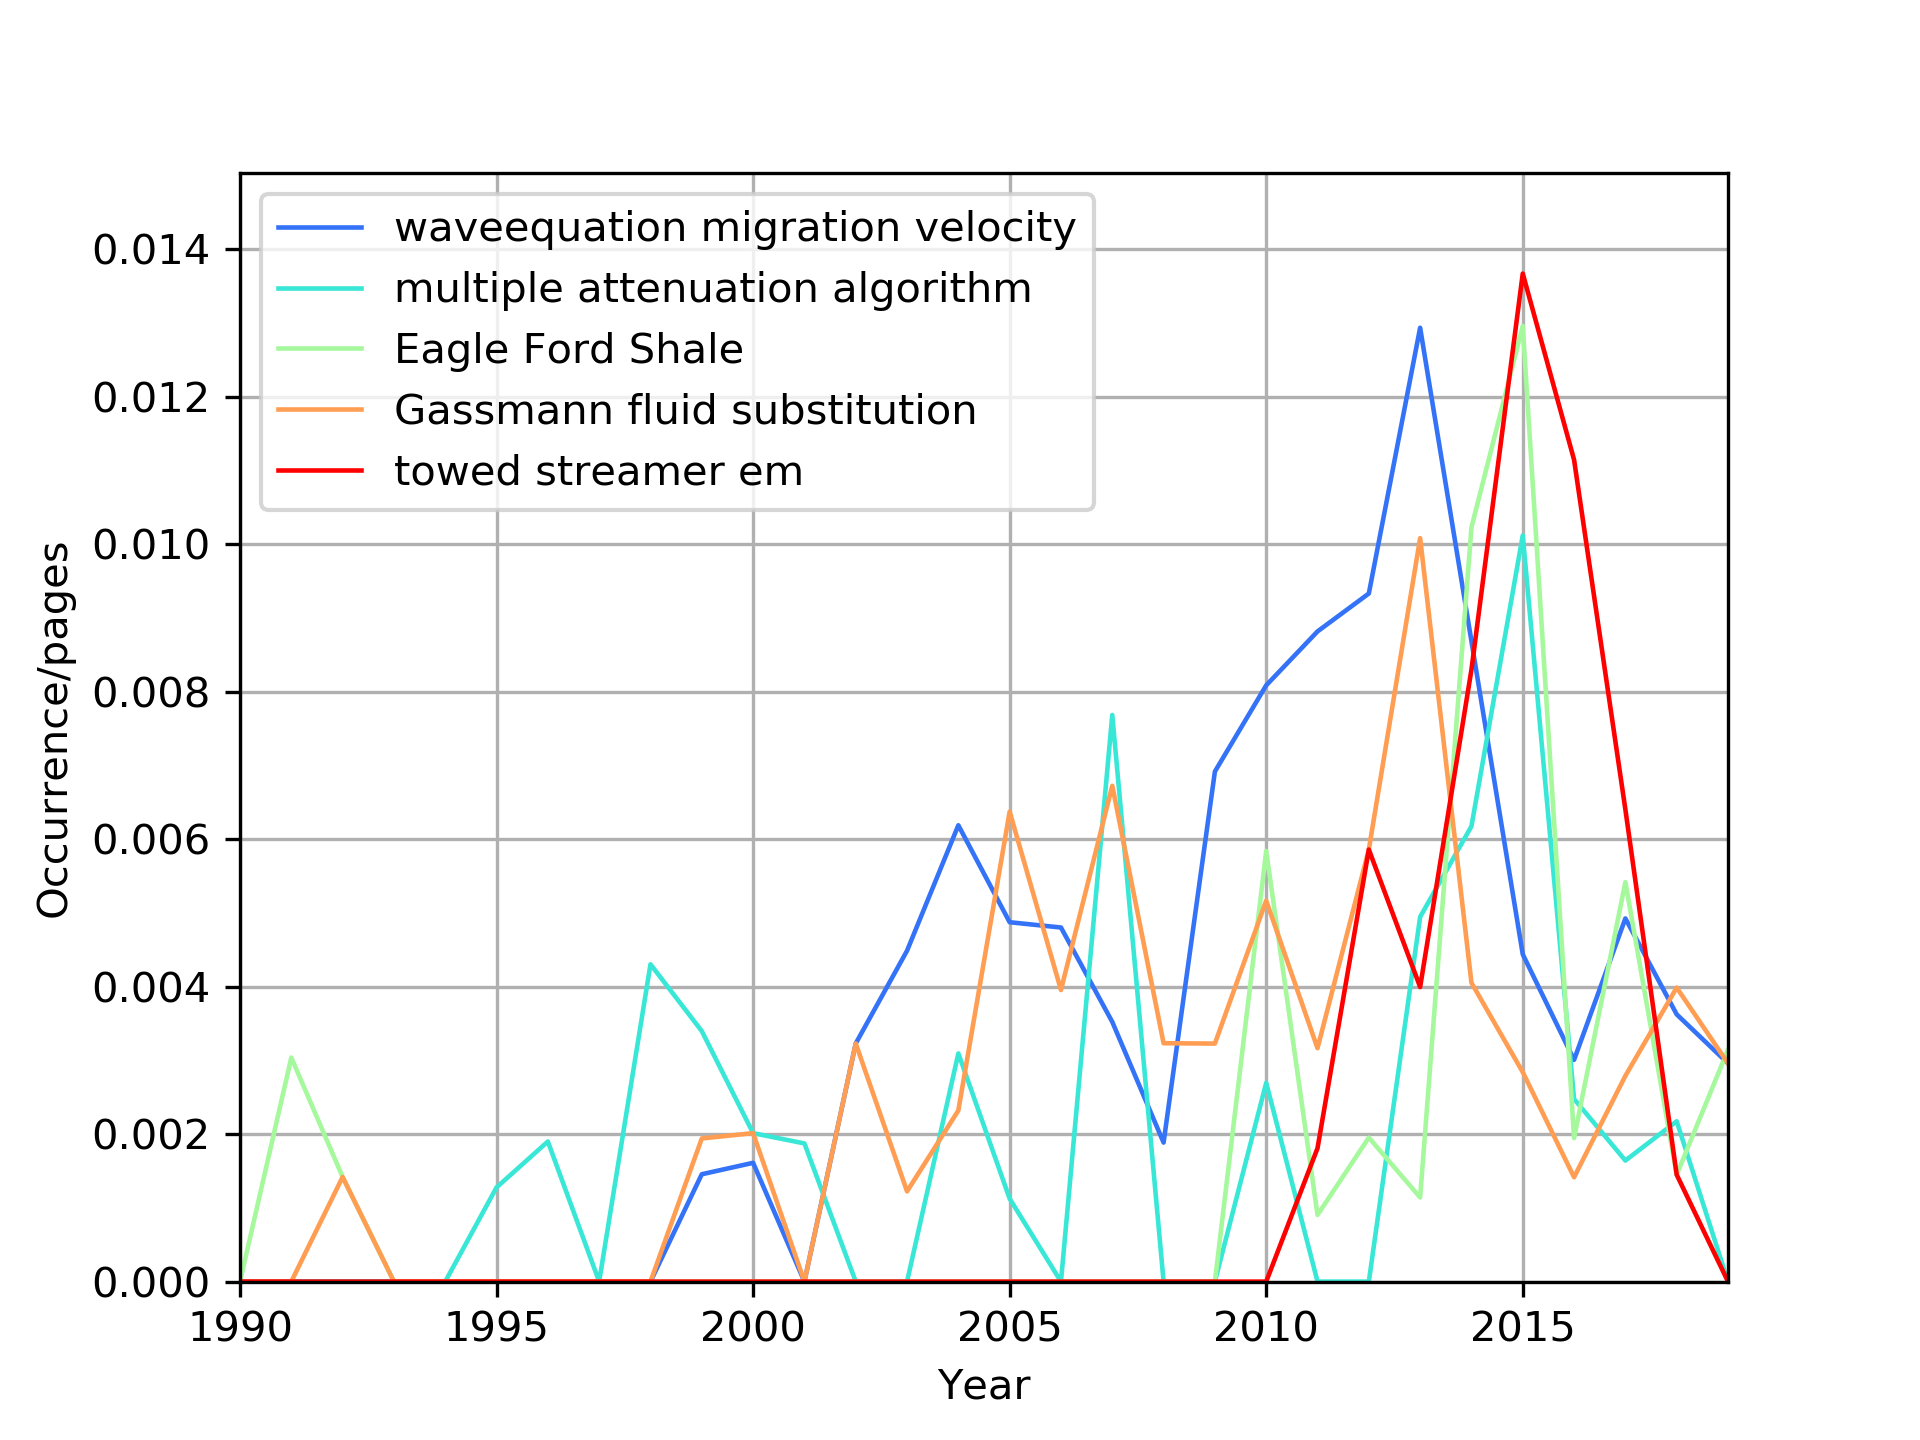
\includegraphics[clip,width=1\linewidth]{most_decl_tri.png} }
\end{minipage}

\caption{Three-words phrases that shows the highest rate of occurrence growth (left)  and decline (right) in the past four years.}
\label{trigrams}
\end{figure}

Let us consider most growing and declining three-word phrases, Fig. \ref{trigrams}. The fastest growth shows "convolutional neural network" (CNN), second one is "distributed acoustic sensing" (DAS), which is related to fiber-optic measurement system. In the recent few years researches are using CNN to perform "seismic facies classification", that is why we observe an increase in usage. We also see a relative increase for "ground penetration radar", however, we see that this term was often used during the 90s and early 2000. Right part of Fig. \ref{trigrams} shows decrease in the use of certain seismic terms as for the case of two-word phrases and the name of the shale deposit. From 2010 to 2019, we observe an increase and decrease in interest in the "towed streamer EM".Towed streamer electromagnetic systems allow to collect data with a high rate and over huge survey area, \citep{Zhdanov2015}. But in order to carry out work on wide areas, it is necessary to have the corresponding survey objects, which are now in short supply, therefore we see a decrease in the use of this term.


Of three-words phrases the most frequent now is “full waveform inversion” (Fig. \ref{fwi_psdm}) and it is still growing together with abbreviation “fwi,” the second one is “reverse time migration,” the top three closes “convolutional neural network.” Fig. \ref{fwi_psdm} shows how the occurrence of “prestack depth migration” was substituted by “full waveform inversion” and “reverse time migration.” The frequency of occurrence is higher if we will consider used abbreviations. It is interesting to note that abbreviation “fwi” and “rtm” is used more often than for “psdm” even when it was much more accessible. Perhaps this suggests a tendency to reduce and simplify the terms, which confirms the reduction in the average length of the words used mentioned earlier. Fig. \ref{fwi_psdm} indicates the emergence of new methods and their development.  The growth of the use of some terms inevitably supplants other words, provided that the volume of published material is approximately the same. During the history of observation, we found many terms that were popular before, but do not find application in the modern world. We hope that in spite of the unprecedented growth of interest in neural networks, the development of classical data processing methods will also continue.


\begin{figure}[ht!]

\begin{minipage}{0.49\linewidth}
\center{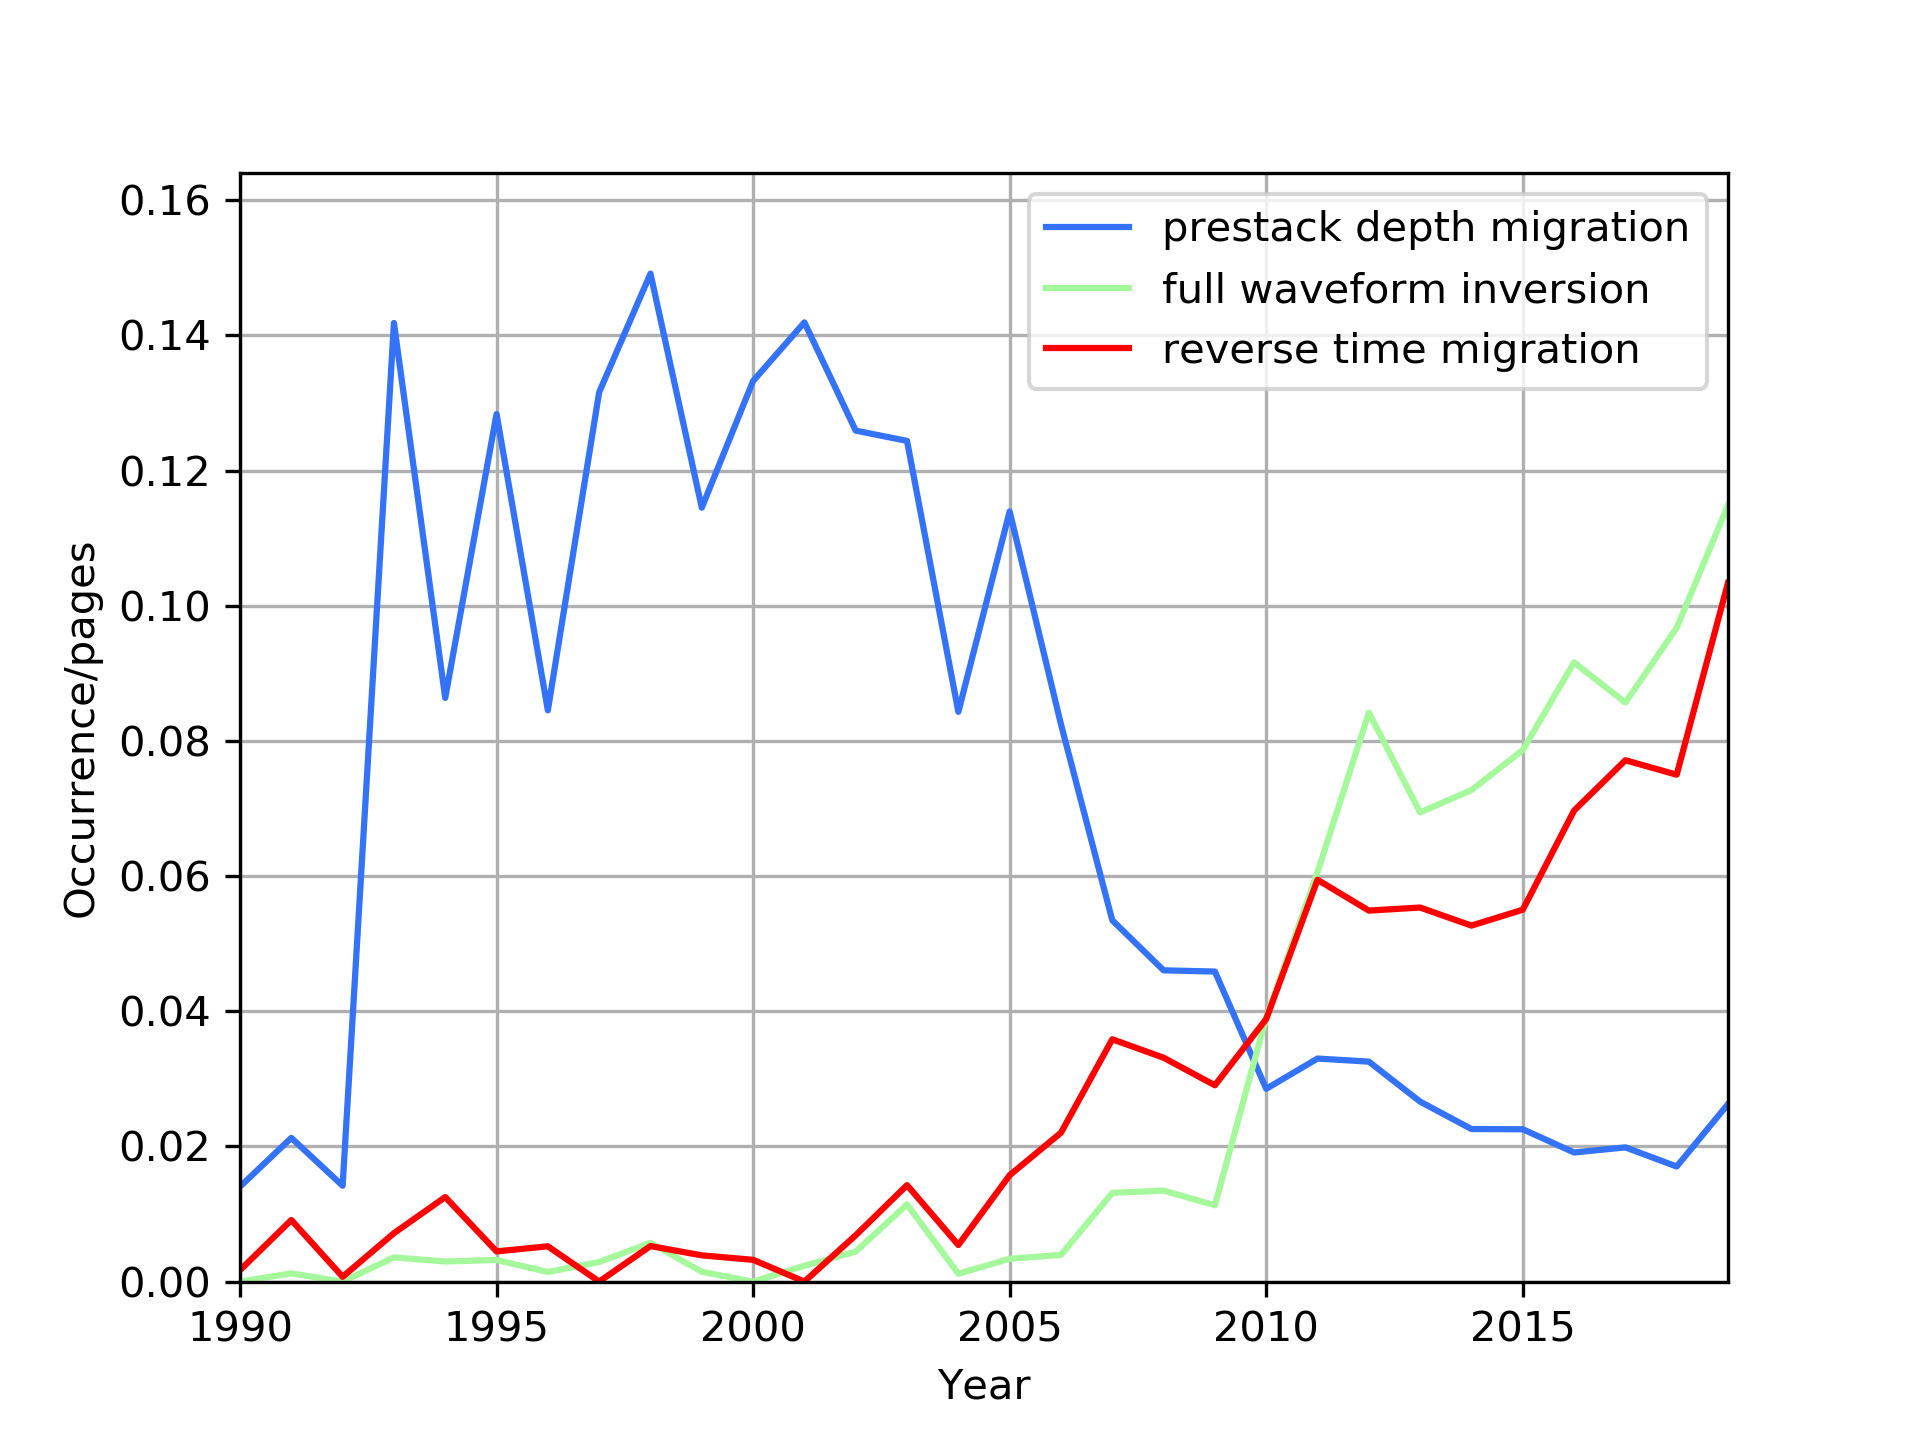
\includegraphics[clip,width=1\linewidth]{fwi_rtm_psdm2.png} }
\end{minipage}
\hfill
\begin{minipage}{0.49\linewidth}
\center{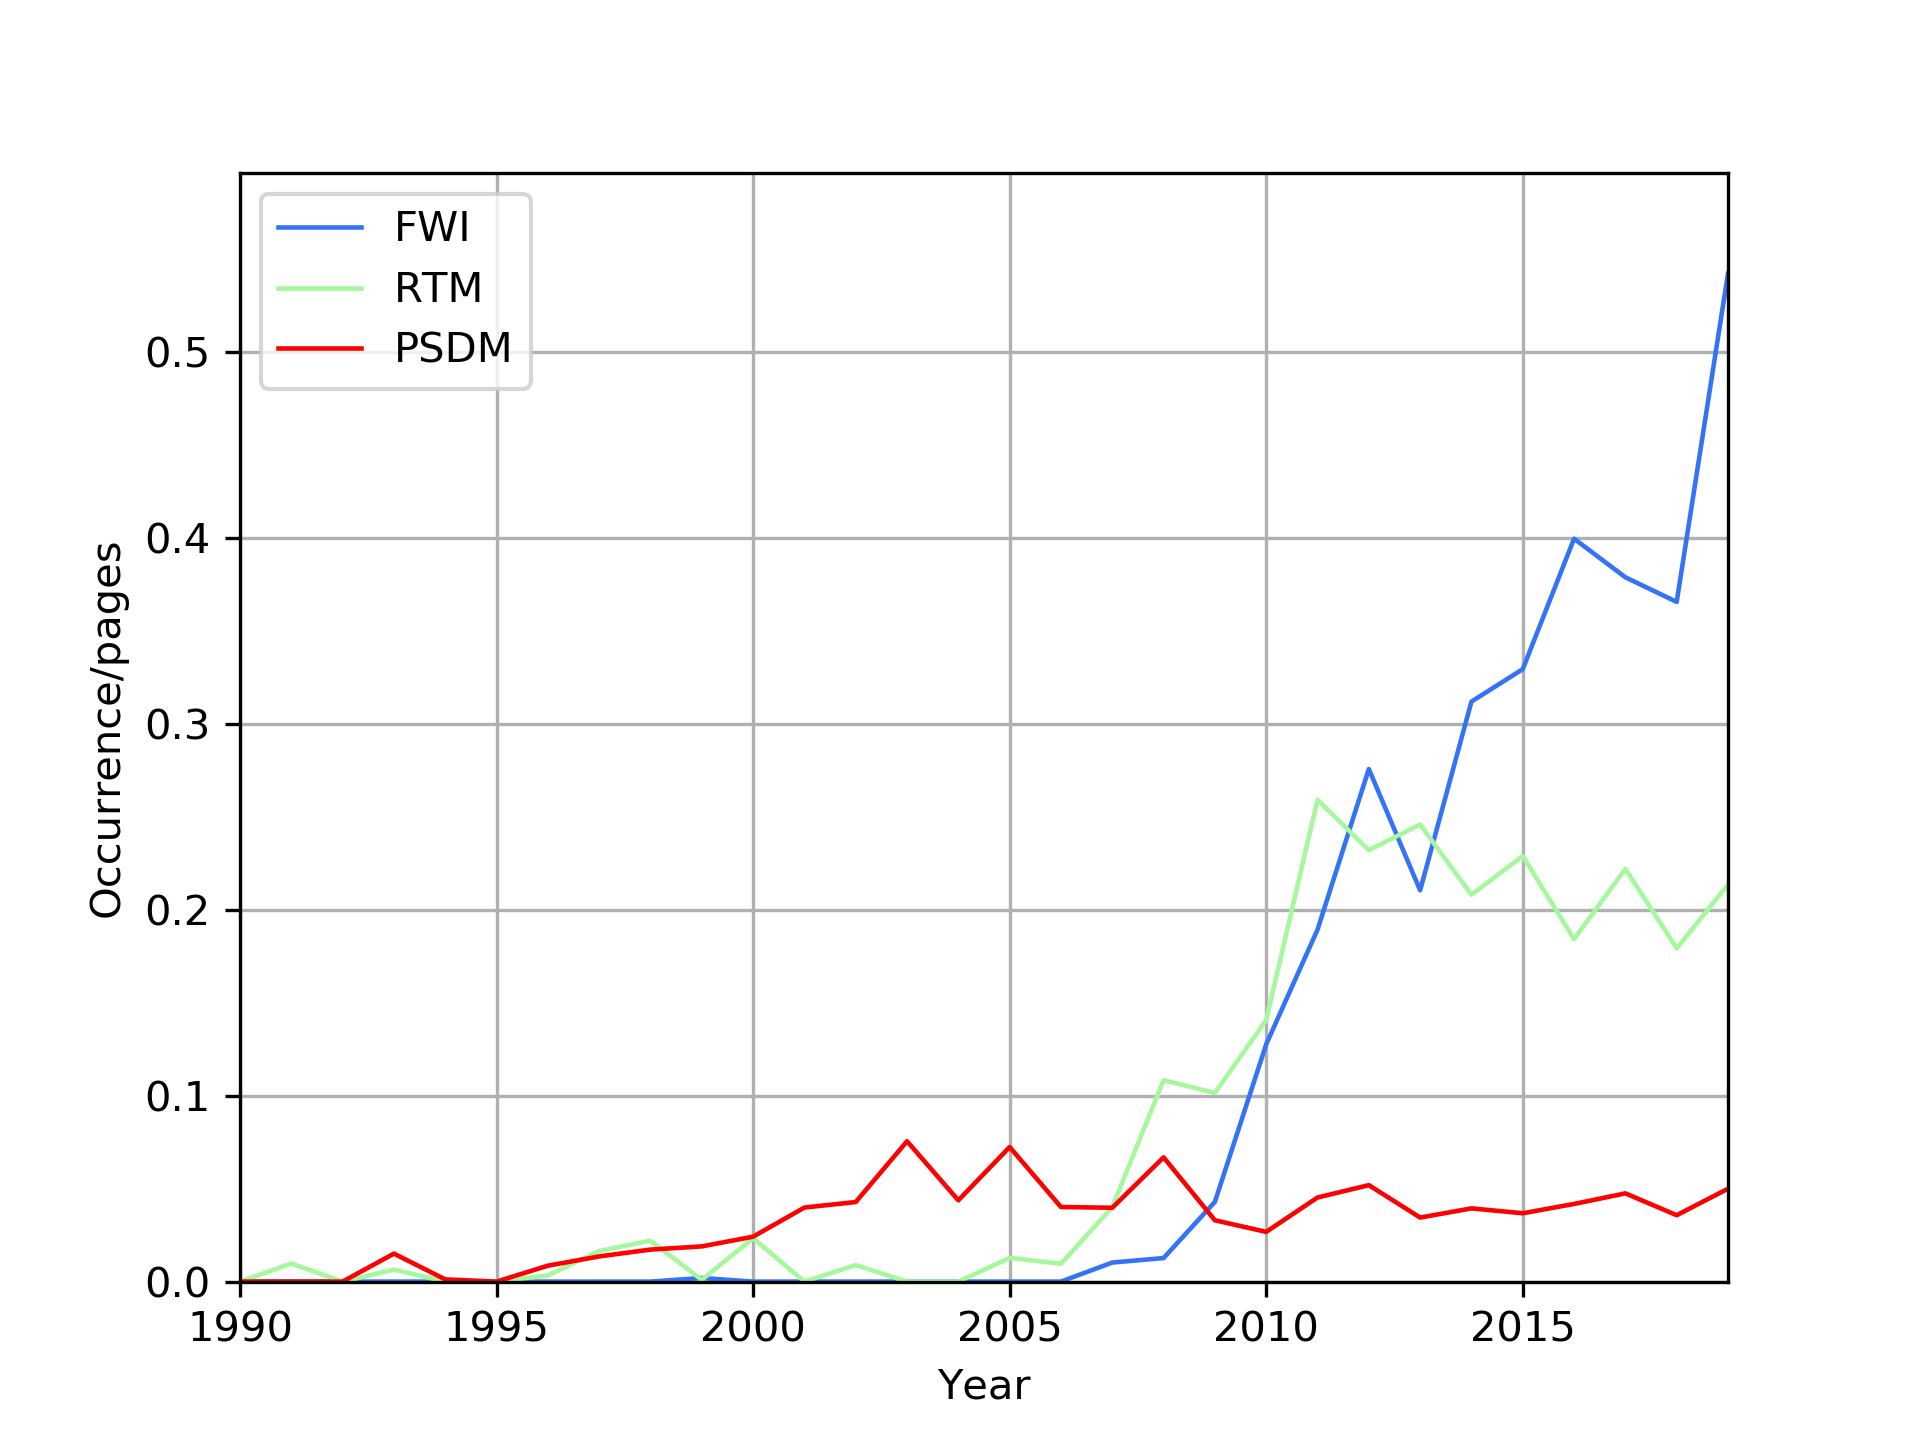
\includegraphics[clip,width=1\linewidth]{fwi_rtm_psdm.png} }
\end{minipage}

\caption{Change in the use of seismic data processing methods: full expression (left) and abbreviations (right).}
\label{fwi_psdm}
\end{figure}


It is curious that in 2018, we observe an increase in the mention of the words “student,” “faculty,” and “researcher.”, Fig. \ref{stu_faculty_mon}, left.  Does this mean that the number of academic impacts has grown in the last year? You may notice a tendency to increase the use of words “engineer” after growing occurrence for word “student”. We observe the growth of occurrence the "researcher" word in past ten years and it appears more often then engineer in 2019. During 1990s we observe more occurrence of word "engineer" in comparison to "researcher" and "scientist", in the past decade the situation changes bringing "researcher" to the first place. On the right of Fig. \ref{stu_faculty_mon} we observe increase in usage of monitoring. For example, this applies to microseismic monitoring and monitoring of the reservoir. The increased use of the term "monitoring" and "efficiency" indirectly indicates the concentration of researchers on the development of already explored deposits. The term "legacy" primarily refers to old data that is reprocessed using modern methods including CNN. It is interesting that in the 1980s we used the word "future" more often than now, perhaps, we can agree, the past is over.


\begin{figure}[ht!]

\begin{minipage}{0.49\linewidth}
\center{\includegraphics[clip,width=1\linewidth]{stu_faculty.png} }
\end{minipage}
\hfill
\begin{minipage}{0.49\linewidth}
\center{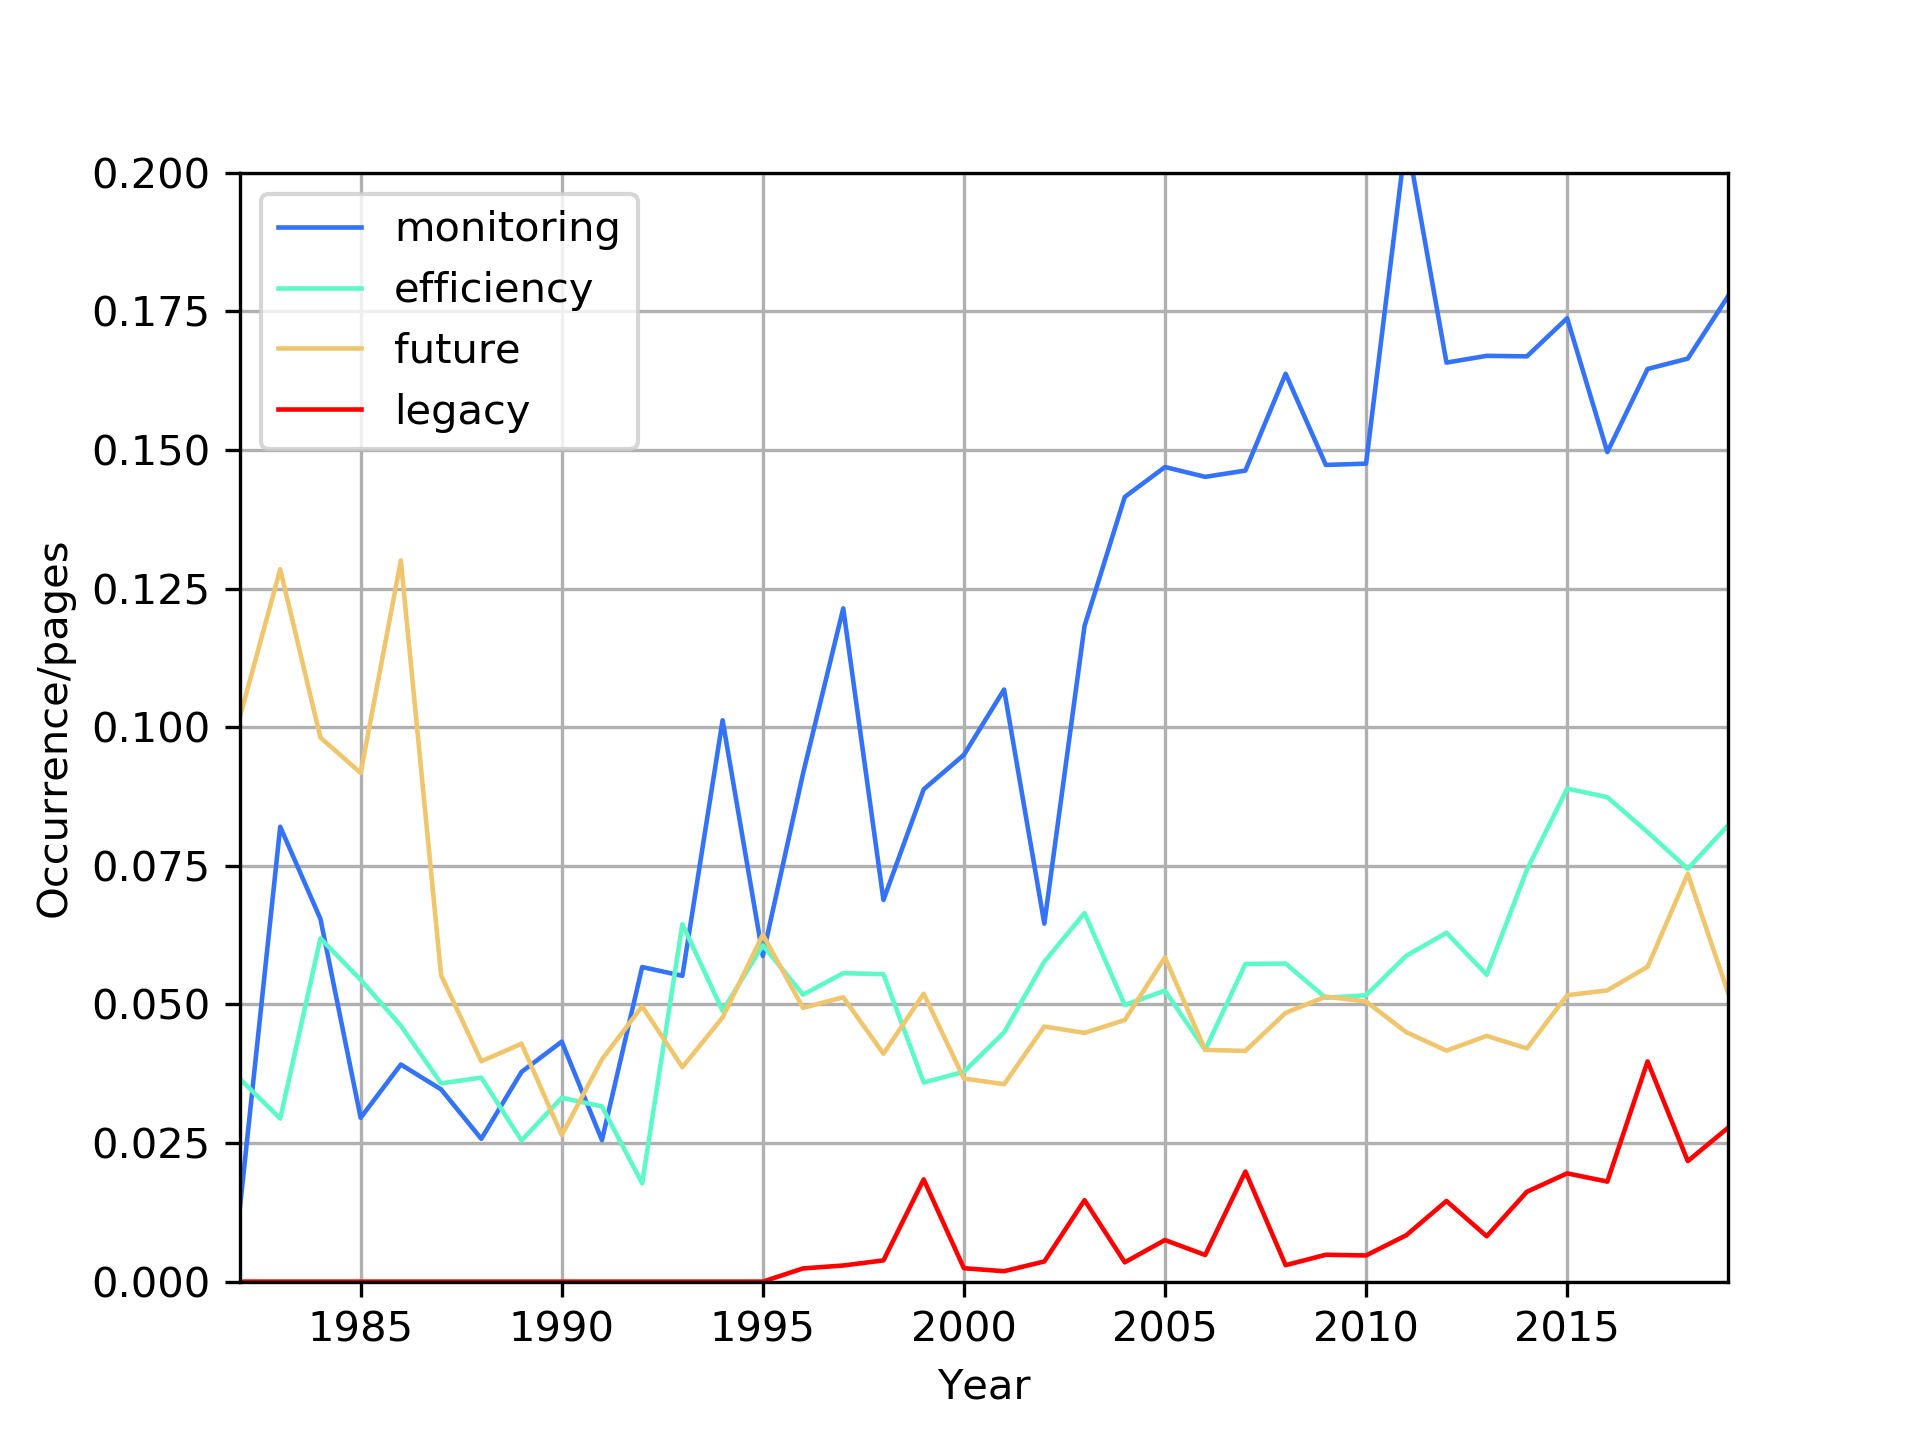
\includegraphics[clip,width=1\linewidth]{sigrams_int2.png} }
\end{minipage}
\caption{Change in word usage over time.}
\label{stu_faculty_mon}
\end{figure}


%%%%%%%%%%%%%%%%%%%%%%%%%%%%%%%%%%%%%%%%%%
\section{Discussion}

The emergence of new techniques in geophysics inevitably leads to an increase in the use of terms from this field. The frequency of words used can be used to track trends in the emergence of new equipment, processing methods, math algorithms, and types of resources being developed, including oilfields and kind of rocks being studied. The amount of hidden information is astounding. Such a study is unique because we have at our disposal a history of the development of geophysics. And it allows us to track exactly how the professional language changes over time.

We see that usually the growth in the use of the terms is saw tooth like, it is non monotonic with individual peaks. In fact, each peak represents the next phase of implementation, new research objects and new teams that have mastered the method. A qualitatively different picture is observed with "neural networks". From 1990 to the beginning of 2000, attempts were made to use neural networks in geophysics, but they were suspended until 2016, in which a rapid growth in the use of this and related terms began. On average, we find "neural network" phrase on every fourth page of conference materials. If we observe an increased interest in this topic, then the researchers sincerely believe that using the methods of machine learning can solve many problems of geophysics. Is the automation of the interpreter the main problem of modern geophysics? The authors believe that the main problem of geophysics now is the lack of new research objects, hydrocarbon and other mineral deposits, and this is the reason for the increased interest in the development of methods for automatic processing of geophysical data. At the same time, the use of such words as "monitoring" and "efficiency" is growing, which indicates an understanding of the need for a more complete extraction of hydrocarbons and monitoring of developed fields.


\begin{figure}[ht!]
\centering
\includegraphics[scale=1]{2019_w_bg.png}
\caption{Word cloud for SEG Annual Conference and Exhibition 2019. 200 most frequently used words, size of the word corresponds to relative number of usage.}
\label{2019_w_bg}
\end{figure}


Exploring the use of terms at the SEG Annual Conferences, we mainly studied the seismic trend in geophysics (see ). Even a brief look at Fig. \ref{2019_w_bg} give the understanding about main focus of the SEG Annual Conferences nowadays. Perhaps building similar word clouds for other conferences will provide a clearer picture of them. However, it would be interesting how other methods are developing in geophysics: downhole methods, electrical exploration methods, petrophysics, engineering geophysics, etc. For this, it is worthwhile to study the materials of conferences and publications of other journals with a different specialization. Research of conferences materials of other societies (SPWLA, EAGE, SPE) will provide a complete picture of the oil industry development.

The authors believe that the resulting database of industrial organizations and universities can be used to study the oilfield services and oil production market, or by students when searching for a place to study. We encourage readers to use our data available online (link). The data includes filtered word lists with the frequency of use in each year, the number of pages and the average number of co-authors. Thus, the reader will be able to conduct their own research, test their hypotheses or assumptions.


%%%%%%%%%%%%%%%%%%%%%%%%%%%%%%%%%%%%%%%%%%
\section{Conclusions}

We analyzed 24,500 papers including 106,500 pages consisting of 57 million words, or more than 383 million symbols. Change in the professional language reflects the change in the industry and science.  USA academia has the biggest impact in the proceedings of SEG Annual Conference during the whole observation period. We observe that the number of Chinese academia affiliations is growing, reaching the USA academia affiliations number. Representing companies at the SEG Annual Conference practically shows the economic condition of the company. Proposed tool can be used by investors for profit. And students of geophysics will be able to choose the right university for study, looking at our results on the geography of geophysical academia. “Neural network” and related disciplines show the fastest growth in the last two years. The authors doubt that growth will continue at the same rate as the term “neural network” is already used more than the term “field data” in 2018. More likely “neural network” related disciplines will occupy its niche in geophysics for the upcoming years. We also observe the rapid growth of the word “fiber,” which is more likely related to fiber optic sensing systems. Supposedly, we will see more projects on “monitoring” of oil and gas fields and increasing production “efficiency,” while there will be less work on the exploration of new fields.


%%%%%%%%%%%%%%%%%%%%%%%%%%%%%%%%%%%%%%%%%%
\vspace{6pt} 

%%%%%%%%%%%%%%%%%%%%%%%%%%%%%%%%%%%%%%%%%%
%% optional
%\supplementary{The following are available online at \linksupplementary{s1}, Figure S1: title, Table S1: title, Video S1: title.}

% Only for the journal Methods and Protocols:
% If you wish to submit a video article, please do so with any other supplementary material.
% \supplementary{The following are available at \linksupplementary{s1}, Figure S1: title, Table S1: title, Video S1: title. A supporting video article is available at doi: link.}

%%%%%%%%%%%%%%%%%%%%%%%%%%%%%%%%%%%%%%%%%%
\authorcontributions{Data mining and processing, software development and analysis, original draft preparation - Timofey Eltsov; software development and analysis, review and editing of the draft - Maxim Yutkin; supervision, project administration, historical analysis, review and editing of the draft - Tadeusz W. Patzek.}

%%%%%%%%%%%%%%%%%%%%%%%%%%%%%%%%%%%%%%%%%%
\funding{Dr. Eltsov was supported by the KAUST Magnetic Sensor project, REP-2708.}

%%%%%%%%%%%%%%%%%%%%%%%%%%%%%%%%%%%%%%%%%%
\acknowledgments{Authors appreciate the responsiveness of the SEG team for permission to use digital data and especially SEG Digital Publications Manager, Jeno Mavzer for useful advice and help. We would like to acknowledge Dr. Charles Russell Severance for informative Python course.}

%%%%%%%%%%%%%%%%%%%%%%%%%%%%%%%%%%%%%%%%%%
\conflictsofinterest{The authors declare no conflict of interest.} 

%%%%%%%%%%%%%%%%%%%%%%%%%%%%%%%%%%%%%%%%%%
%% optional
\abbreviations{The following abbreviations are used in this manuscript:\\

\noindent 
\begin{tabular}{@{}ll}
CNN & Convolutional Neural Network \\
DAS & Distributed Acosutic Sensing \\
FWI & Full waveform inversion\\
PSDM & Prestack depth migration\\
SEG & Society of Explorational Geopysicists\\
\end{tabular}}

%%%%%%%%%%%%%%%%%%%%%%%%%%%%%%%%%%%%%%%%%%
%% optional
\appendixtitles{no} %Leave argument "no" if all appendix headings stay EMPTY (then no dot is printed after "Appendix A"). If the appendix sections contain a heading then change the argument to "yes".
%\appendix
%\section{}
%\unskip
%\subsection{}
%The appendix is an optional section that can contain details and data supplemental to the main text. For example, explanations of experimental details that would disrupt the flow of the main text, but nonetheless remain crucial to understanding and reproducing the research shown; figures of replicates for experiments of which representative data is shown in the main text can be added here if brief, or as Supplementary data. Mathematical proofs of results not central to the paper can be added as an appendix.
%%
%\section{}
%All appendix sections must be cited in the main text. In the appendixes, Figures, Tables, etc. should be labeled starting with `A', e.g., Figure A1, Figure A2, etc. 

%%%%%%%%%%%%%%%%%%%%%%%%%%%%%%%%%%%%%%%%%%
\reftitle{References}

% Please provide either the correct journal abbreviation (e.g. according to the “List of Title Word Abbreviations” http://www.issn.org/services/online-services/access-to-the-ltwa/) or the full name of the journal.
% Citations and References in Supplementary files are permitted provided that they also appear in the reference list here. 

%=====================================
% References, variant A: external bibliography
%=====================================
%\externalbibliography{yes}
%\bibliography{your_external_BibTeX_file}
%\bibliography{timaref}
%=====================================
% References, variant B: internal bibliography
%=====================================
\begin{thebibliography}{999}
\providecommand{\natexlab}[1]{#1}

\bibitem[Glauner \em{et~al.}(2018)Glauner, Valtchev, and State]{Glauner2018}
Glauner, P.; Valtchev, P.; State, R.
\newblock {Impact of Biases in Big Data}.
\newblock  In~Proceedings of the European Symposium on Artificial Neural Networks, Computational Intelligence and Machine Learning,  Bruges, Belgium, 25-27 April~2018; pp 645--654.

\bibitem[Kaplan \em{et~al.}(2014)Kaplan, Chambers, and Glasgow]{Kaplan2014}
Kaplan, R.; Chambers, D.A.; Glasgow, R.E.
\newblock {Big Data and Large Sample Size: A Cautionary Note on the Potential for Bias}.
\newblock {\em CTS Journal} {\bf 2014}, {\em 7}, {4}, ~342--346.
\newblock
  doi:{\changeurlcolor{black}\href{ https://doi.org/10.1111/cts.12178}{\detokenize{10.1111/cts.12178}}}.

\bibitem[SEG, (2019)]{SEG}
\newblock {SEG Technical Program Expanded Abstracts. Available online: https://library.seg.org/series/segeab (Accessed on  2 December 2019)}.

\bibitem[OnePetro, (2019)]{SPE2019}
\newblock {OnePetro online library. Available online: https://www.onepetro.org (Accessed on  2 December 2019)}.

\bibitem[American Higher Education Hits a Dangerous Milestone, (2018)]{Brownstein2018}
\newblock {American Higher Education Hits a Dangerous Milestone}. \newblock {Available online: https://www.theatlantic.com/\\politics/archive/2018/05/american-higher-education-hits-a-dangerous-milestone/559457/ (Accessed on  2 December 2019)}
%author = {Brownstein, Ronald},
%shorturl.at/PRWYZ (Accessed on  2 December 2019)}.

\bibitem[Mallapaty (2018)]{Mallapaty2018}
\newblock {Paper authorship goes hyper. Available online: https://www.natureindex.com/news-blog/paper-authorship-goes-hyper (Accessed on 17 October 2019)}.

\bibitem[ExxonMobil(2014)]{ExxonMobil2014}
ExxonMobil.
\newblock {\emph{Summary Annual Report 2014}};
\newblock Report; {ExxonMobil: Irving, TX, USA,}  2014.

\bibitem[Trainor-Guitton \em{et~al.}(2018)Trainor-Guitton, Jreij, Guitton, and Simmons]{Trainor-Guitton2018}
Trainor-Guitton, W.; Jreij, S.; Guitton, A.; Simmons, J. 
\newblock {Fault classification from 3D imaging of vertical DAS profile}.
\newblock  In~Proceedings of the SEG Annual Conference and Exhibition,  Anaheim, USA, 14-17 October~2018; pp 4664--4668.

\bibitem[Binder and Chakraborty(2018)]{Binder2019}
Chakraborty, G.; Chakraborty, D. 
\newblock {Detecting microseismic events in downhole distributed acoustic sensing data using convolutional neural networks}.
\newblock  In~Proceedings of the SEG Annual Conference and Exhibition,  San Antonio, USA, 15-20 September~2019; pp 4864--4868.

\bibitem[Lomas and Curtis(2014)]{Lomas2019}
Lomas, A.; Curtis, A.
\newblock {An introduction to Marchenko methods for imaging}.
\newblock {\em Geophysics} {\bf 2019}, {\em 84}, {2}, ~35--45.
\newblock
  doi:{\changeurlcolor{black}\href{ https://doi.org/10.1190/geo2018-0068.1}{\detokenize{10.1190/geo2018-0068.1}}}.

\bibitem[Penna \em{et~al.}(2019)Penna, Ara{\'{u}}jo, Geisslinger, Sansonowski, Oliveira, Rosseto, and Matos]{Penna2019}
Penna, R.; Ara{\'{u}}jo, S.; Geisslinger, A.; Sansonowski R.; Oliveira, L.; Rosseto J.; Matos, M.
\newblock {Carbonate and igneous rock characterization through reprocessing , FWI imaging , and elastic inversion of a legacy seismic data set in Brazilian presalt province}.
\newblock {\em The Leading Edge} {\bf 2019}, {\em 38}, {1}, ~11--19.
\newblock
  doi:{\changeurlcolor{black}\href{ https://doi.org/10.1190/tle38010011.1}{\detokenize{10.1190/tle38010011.1}}}.

\bibitem[Hill(1990)]{Hill1990}
Hill, N.R.;
\newblock {Gaussian beam migration}.
\newblock {\em Geophysics} {\bf 1990}, {\em 55}, {11}, ~1416--1428.
  doi:{\changeurlcolor{black}\href{https://doi.org/10.1190/1.1442788}{\detokenize{10.1190/1.1442788}}}


\bibitem[Huang \em{et~al.}(2001)Huang, Sherrill, and Sengupta]{Huang2001}
Huang, S.; Sherrill, F.; Sengupta, M.K. 
\newblock {Merits of amplitude preserving Kirchhoff beam migration method for 3D AVO analysis}.
\newblock  In~Proceedings of the SEG Annual Conference and Exhibition,  San Antonio, USA, 9-14 September~2001; pp 1--4.

\bibitem[Ting and Wang(2008)]{Ting2008}
Ting, C.O.; Wang, D.
\newblock {Controlled beam migration applications in Gulf of Mexico}.
\newblock  In~Proceedings of the SEG Annual Conference and Exhibition,  Las Vegas, USA, 9-14 November~2008; pp 368--372.

\bibitem[Zhdanov \em{et~al.}(2001)Zhdanov, Endo, Sunwall, and Mattsson]{Zhdanov2015}
Zhdanov, M.S.; Endo, M.; Sunwall, D.; Mattsson, J.
\newblock {Advanced 3D imaging of complex geoelectrical structures using towed streamer EM data}.
\newblock  In~Proceedings of the SEG Annual Conference and Exhibition,  New Orleans, USA, 18-23 October~2015; pp 904--908.

\end{thebibliography}
%%%%%%%%%%%%%%%%%%%%%%%%%%%%%%%%%%%%%%%%%%
%% optional
%\sampleavailability{Samples of the compounds ...... are available from the authors.}

%% for journal Sci
%\reviewreports{\\
%Reviewer 1 comments and authors’ response\\
%Reviewer 2 comments and authors’ response\\
%Reviewer 3 comments and authors’ response
%}

%%%%%%%%%%%%%%%%%%%%%%%%%%%%%%%%%%%%%%%%%%
\end{document}

